% !TEX root = ../../book.tex
%\hfill
%\par\vspace{\baselineskip}
\chapter{Modeling Trade Data}\label{chap:ch_trade_data_models}

Many articles and books have appeared on the topic of modeling trade data. There is a wealth of information out there and our goal in this chapter is to review modeling approach commonly practiced in the industry. As in the rest of this book our effort is to provide context on the the role these models play in practice, the challenges and considerations that are involved in dealing with trade data day in and day out and then provide the quantitative foundation the reader needs to progress further. This chapter follows the same pattern as used in other parts of this book. We start with a practitioner's view of the subject, what approaches are used  and why and discuss some intuitive ideas on how to tackle these problem. We look at the need and importance of normalization analytics and their role in execution algorithms. We'll go into some details on the most important analytics and ideas on common modeling approaches. We then turn to a review of common microstructure signal that are commonly used in HFT and execution as foundation for more advance alpha signals. We then provide for a more in-depth quantitative treatment on some of the sophisticated models discussed in applied and academic research areas. \\


\noindent\textbf{On Data Preparation:} Before we delve into detail, it's important to discuss an area, often completely disregarded when creating production quality analytics---the data preparation. This step is clearly important in any modeling but for trading this is of particular interest. Trading is a highly behavioral process and as such it's patterns have strong seasonal component due to financial events and specific moments of the corporate life-cycle. During these periods often called ``special days'' the behavior of the stock have strong variation from regular days and should be excluded when general analytics are created and special days analytics should be created separately. Examples of special days include: Futures and Options expiration days, FOMC announcements, earnings announcements, etc.. While this appears to be a simple process, in practice maintaining special day calendar can be a source of some manual labor. It has to be observed sometimes it is not the quantitative aspects that end up being the hardest problem to solve.



\section{Normalizing Analytics}

A challenging aspect of execution, unlike other areas in algorithmic trading, is developing strategies that apply to a large number of stocks. The strategies will need to function successfully for from super liquid instruments that trade easily at the minimum tick size, to illiquid stocks that trade only infrequently at wide spreads. These include stocks that have very stable and large sizes at the inside market, and stocks whose NBBO (best bid-best offer) changes almost every second.


To complicate matters further the above characteristics, it should be noted, do not remain constant. Intra-day trading variations are well documented and are firmly rooted in institutional investor behavior. Immediately after the open there is a lot of trading activity as investor incorporate the information from overnight news. The increased uncertainty on the stock valuation is reflected by a much higher volatility and spread in the early trading hours. Once the (often called) price discovery period is over (usually within 15--30~m in US markets), the trading behavior settles in and activity is reduced and so do spreads and volatility. Activity then resumes towards the end of the day in particular due to the  fact that many active funds are marked to the day's closing price. European markets have further predictable ``bumps'' in and around the US market open as the markets absorbs the reaction of US investors.


As mentioned there are also important sources of inter-day variability with the impact of special days. For  example the trading activity during futures/options expiration is heavily tilted towards the close since the settlement prices are related to the closing price on that day. On Fed announcement days trading activity slows to a tick ahead of the announcement as investor await any surprise decision. Activity jumps immediately after that, incorporating any relevant information.


The complexity of dealing in a systematic way all the above variability is a daunting task. One could (and in some cases arguably should) apply different approaches to achieve the same benchmark for different types of stocks and different days or time of day but that is never done in practice as it would be completely unwieldy and the system would be prohibitively expensive to build and maintain. How is this addressed? The practitioner's approach is to parametrize many of the trading decisions using normalizing features, variables that help adapt the trading decision to a particular situation.


The next section provides a brief review of the most commonly used analytics and gives pointers to some modeling approaches. This subject is quite broad and, while extremely important in practice, has gotten little attention in academic research. We will only provide a relatively coarse treatment of the subject from a practitioner's perspective. It should be sufficient as a starting point for anyone to build  the necessary analytics for a basic Execution Algo.



\subsection{Order Size Normalization: ADV}

Assume a trader needs to execute an order for one million shares of XYZ. If an order is a big order it has to be carefully managed or a tiny order the trader can simply ``fire and forget''.  Intuitively, from trading perspective, due to  the large difference in stock characteristics and in liquidity, order size should be viewed as a relative measure. The most commonly used order size normalizer is the Average Daily Volume (ADV). While the term ADV has a simple connotation, it is actually a very important measure for order sizing, position limit, etc., and there are some considerations and decisions to make: which location measure to use---average, median, some other measure robust to outliers? Over what horizon? How to treat special days? The answer is likely to be application specific and there is very little consensus or systematic study on the use of different measures.\footnote{One of the authors spent several months running a project aimed at standardizing all systems to use one ADV measure, when there were 5 in production at the same time!}
 	
	\begin{figure}[!ht]
		\centering
			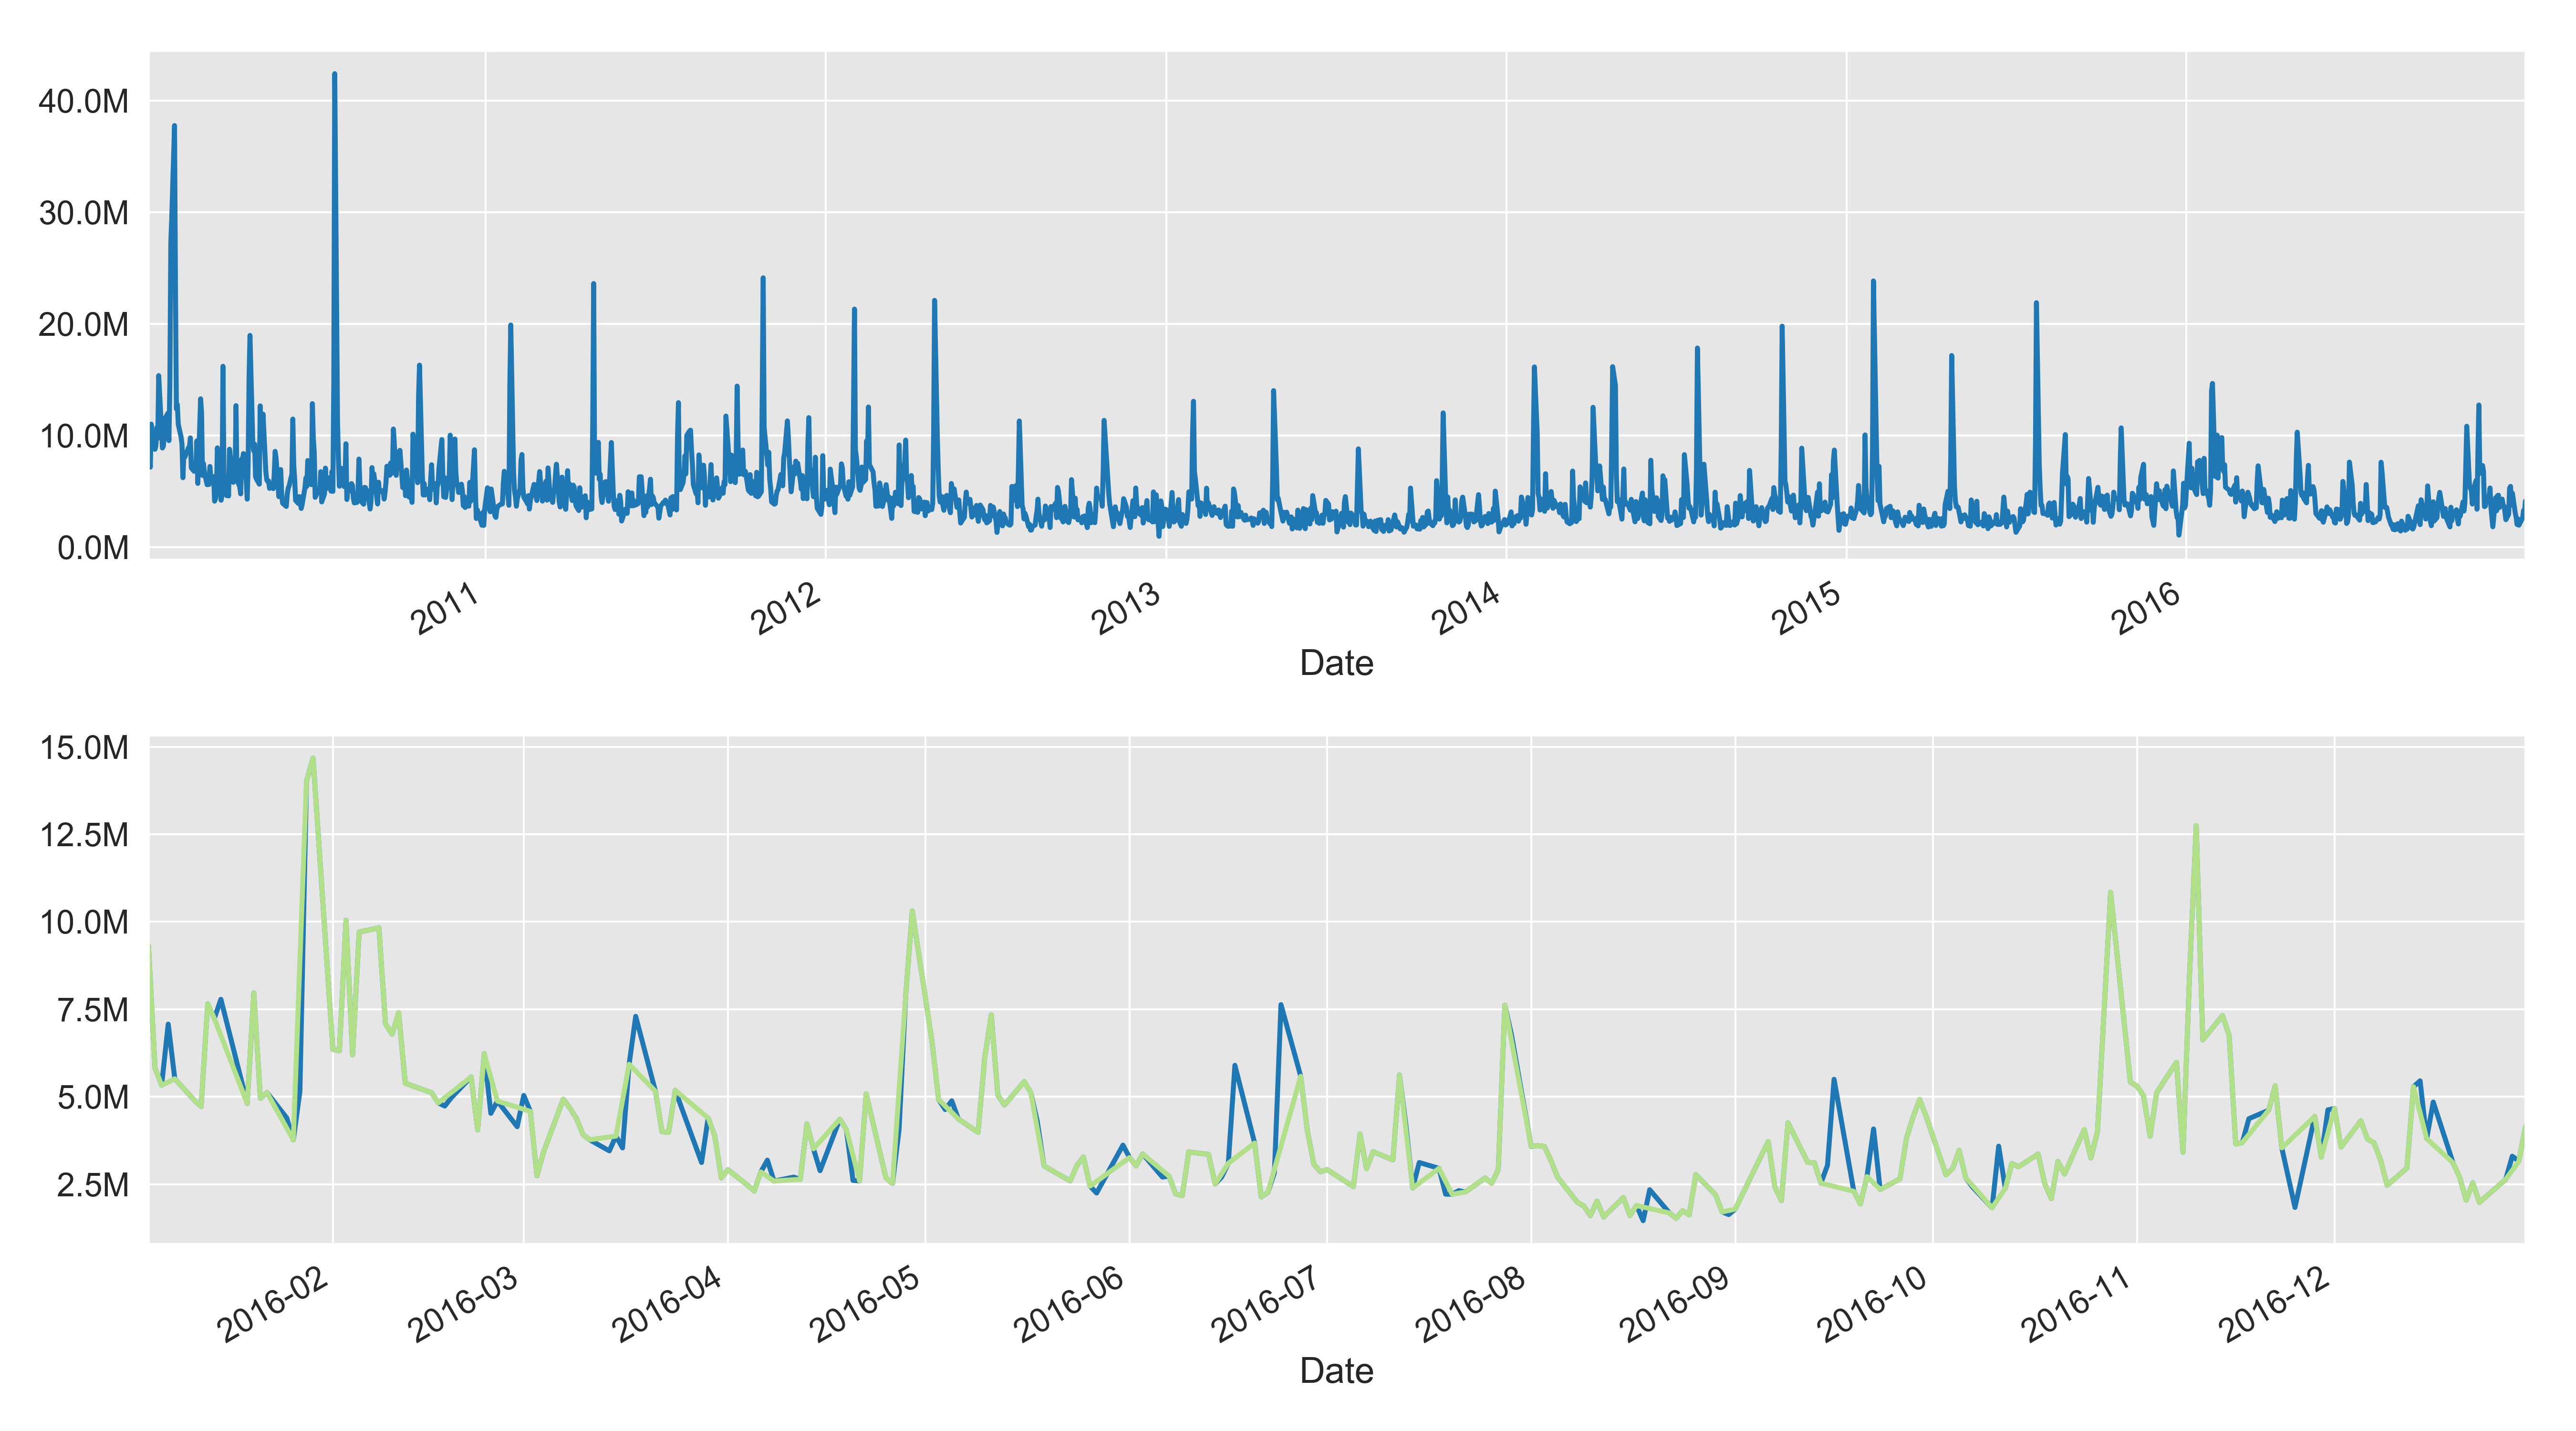
\includegraphics[width=0.75\textwidth]{chapters/chapter_trade_data_models/figures/daily_volume.png} 
		\caption{Amazon Daily Volume. \label{fig:daily_volume}}
	\end{figure}
	
Notice how volatile the data is from Figure~\ref{fig:daily_volume}. The volume is strongly autocorrelated with periodic predictable spikes for special days and unpredictable `surprises.' As a baseline metric, the 64 days' mean or median daily volume are probably the most commonly used metric in the industry as the time horizon covers a full quarterly earning cycle and thus it's viewed as incorporating all the seasonal effects of the daily volume. See the graphs (Figure~\ref{fig:adv}) below.
	
	\begin{figure}[!ht]
		\centering
			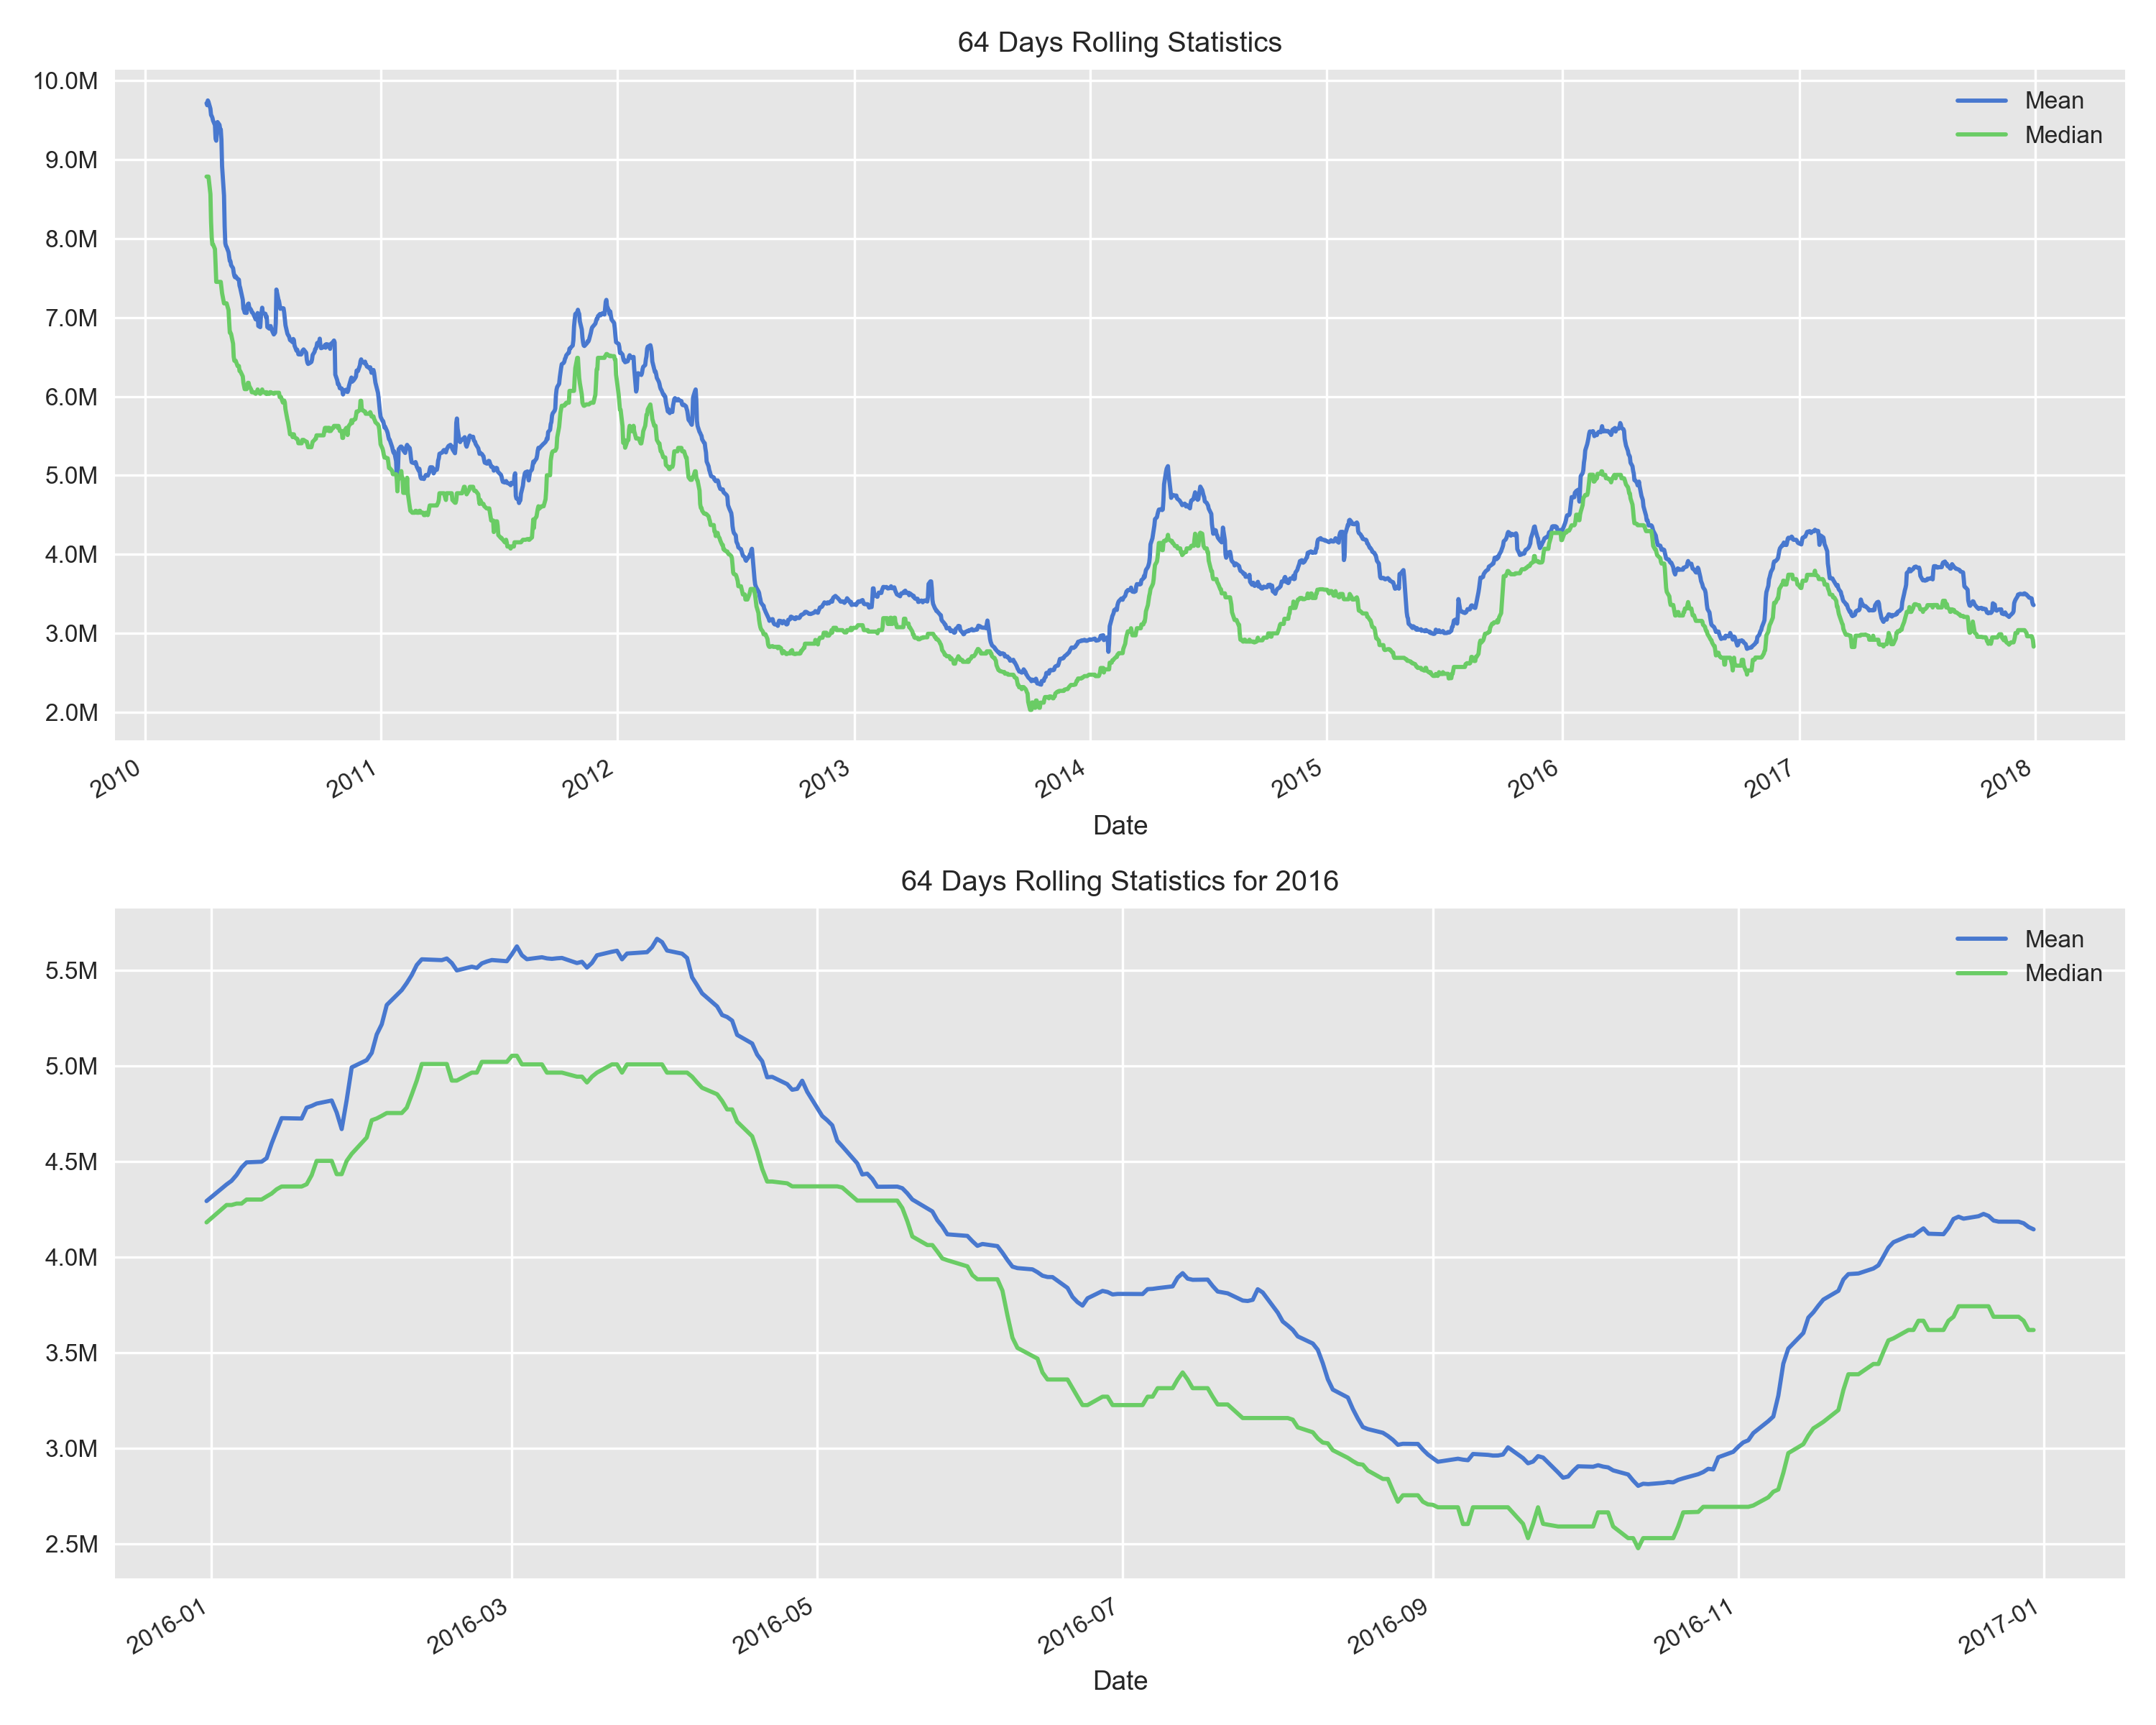
\includegraphics[width=0.75\textwidth]{chapters/chapter_trade_data_models/figures/adv.png} 
		\caption{Average Daily Volume.\label{fig:adv}}
	\end{figure}
Notice how the two measures differ. The median is more stable and smooth but the average is more reactive. Which one to use depends on the application. Note in this section we discussed only about normalizing the volume and not the prediction aspects. These two quantities are used differently. A common use of relative order size is, as we will see in Chapter~10, in the calibration of a market impact model. One would intuitively think that because the calibration is done ex-post it should be normalized using the realized daily volume instead of the ADV. Empirical research has shown that this approach leads to somewhat poorer predictions. It is possible that the large-noise-to-signal ratio is better adjusted by a more stable normalizer in place for a more noisy but more precise one. For consistency reasons because we use ADV as normalizer in the calibration it is often suggested to use of the same normalizer when used for market impact estimation rather than using our best prediction of daily volume. This can be problematic in particular on days where the volume is predictably higher. Practitioners are interested in this important issue and some research in this area would be of practical interest. For a discussion on volume weighted average price (VWAP) prediction refer to Brownlees et al. (2011)~\cite{brownless}.



\subsection{Time-scale Normalization:Characteristic Time}

Trading dynamics have an intrinsic time scale that varies significantly across the stock universe. The specifics of the microstructure determine how fast information is incorporated in the stock price and it is often important to take this into consideration. For instance in a trading algorithm, when evaluating a decision on posting vs. taking, we need to estimate the likelihood the order would get executed before we fall behind on our trading commitments. We would not post passively if, on average, it takes three minutes for an order placed at the bottom of the queue to get executed and we only have 30 seconds to complete trade. However posting passively would be appropriate if it takes 15 seconds in average for the queue to turn over. There a several measures that are often used in practice:
        \begin{itemize}
        \item Straight Time: A surprising number of traders completely ignore this and just use the same time interval for all stocks. Simple but definitively it is sub-optimal.
        \item Event/Tick Time: The normalization is done by counting a certain number of events of quote changes (e.g. ten ticks). Often used in HFT, it is probably the most effective method but requires to keep track of every single tick change which is computationally intensive. It is also not easy to conceptualize as the timescale as ten ticks could be microseconds for some stocks and several seconds or more for certain illiquid instruments.
        \item Volume Time: This normalization uses a certain specified amount of volume (e.g. 1000 shares). Coarser than tick time but easier to implement as most algorithms already keep track of how much volume has been traded. It also suffers from similar issues regarding conceptualization.
        \item Turnover/Characteristic Time: This measures the time it takes for the quote to move on average (more often median). In the simplest setting a quote moves when all the liquidity is removed from a level. This would be the time it takes for a passive order to get executed if it is placed on the queue. It's a simple measure since this can be calculated in advance as an historical mean (median). It also represent a time scale, thus making it easy to conceptualize.
        \end{itemize}


\textnote{TO DO: Graph showing the characteristic time for various stocks}

\subsection{Intraday Return Normalization: Mid Quote Volatility}

Time scale normalization is a 'horizontal' normalization (in a price chart the $x$-axis is time) and for an effective normalized approach we also need a 'vertical' normalization i.e. in price space. For instance if we decide to layer the order book as a way to control adverse selection, the order should be spaced in such a way that it exhibits consistent behavior across different stocks. Placing the orders the same distance for all stocks would cause volatile stock to always execute at multiple levels and for stable stocks, the layering would be useless as the deeper orders would rarely get executed. A commonly used normalizing variable is mid-quote volatility in ticks, estimated as the average number of ticks the mid quote moves in a certain time period stated in terms characteristic time. 

\textnote{TO DO (Raja):  Formulate this in mathematical terms}

\textnote{TO DO (Daniel)  Graph showing examples for different liquidity}


\subsection{Microstructure Normalization}

A common aspect of na\"ive trading strategies is trading in an obvious and predictable way. Some high frequency trading (HFT) strategies are trained to spot the presence of large institutional orders so that they can trade ahead of them to build out their inventory that they can then sell (buy) back at higher (lower) prices. Since an execution strategy has to trade it is impossible to remain completely invisible to the watchful eye of predatory strategies, but with some modest care its impact can be minimized. A common approach used to be less conspicuous is to normalize decision so as to avoid changing the distributional characteristics of various microstructure metrics that are usually closely monitored.  Some examples are:
        \begin{itemize}
        	\item Number of trades per second/period: Used as a normalizing variable to control how often one crosses the spread. Noticeable increase in number of trades per second in a certain direction would be read by a predatory strategy as a sign of urgency.
        	\item Average Trade Size: An unusually large print on an exchange or a larger than average block in a dark venue would be easily spotted giving the strategy away. The average trade size can be used as a normalizer to decide on the size to send to take liquidity.  This measure would be different for different types of venue (lit venues, gray venues, dark venues, etc.)
        	\item Average Quote Size: If the decision to trade passively is made, it is important to size the order appropriately. Placing an order that would noticeably change the average size displayed in the inside quote would be interpreted as a directional signal especially if the size creates a strong imbalance in the order book (see later on imbalance).
        \end{itemize}


Other usage of microstructure normalizer is to support decision making by comparing current conditions with historical averages. A couple of examples:
        \begin{itemize}
        \item Spread: When the decision is to close, in that if the spread has to be crossed to take liquidity, if the current spread is a lot larger than historical averages, it may be an incentive to wait a little longer in the hope that the spread closes in; while if the spread is smaller than usual, all else being equal, the spread can be crossed immediately before the spread returns to its historical normal.
        \item Quote Size: Certain popular liquidity seeking strategies look at the far side visible quantity and compare it to the historical distribution. If the size is "rare enough" (usually that depends on the urgency) the strategy would  cross the spread to capture that before it disappears.\footnote{We discussed before the predictive power of book imbalance. One would think that if a larger than usual size appears at the far side it would create a strong imbalance that would push the price in more favorable situation. That is true and the soundness of the approach could be questioned. On the other side if the display size is rare enough it could imply a error or a naive trading decision and the quantity available could be large enough to put the algo ahead of schedule which would allow it to back off and take advantage of better prices without being forced to catch up to the schedule. }
        \end{itemize}



\subsection{Intraday Normalization: Profiles}

Incorporating intraday seasonality is a critical component of any execution strategy. Intraday seasonality arises from primarily behavioral and practical reasons around trading discontinuities such as the open and the close (and the lunch break period in certain Asian markets) and other scheduled events (e.g. the US open for European markets). Information dissemination tends to cluster around such times and so does the trading activity. The intraday variability of the variables affected by this seasonality is so strong that not considering them would lead to severely sub-optimal decision. Thus standard practice is to incorporate intra-day seasonality using normalized profiles, so that the deviations from the expected value are stated in relative terms. While most microstructure variables discussed above showcase some of this seasonality the most used profiles are: (some of these are covered in Chapter~\ref{ch:ch_mvts}). For any particular duration,
\begin{itemize}
	\item Volume Distribution: The percentage of the expected daily volume that will trade.
	\item Volatility Distribution: The percentage of the expected daily return volatility that will  be perceived.
	\item Spread Multiplier: The percentage deviation from the average spread.
\end{itemize}
Of particular importance is the Volume Distribution (or daily profile) as it is used to create a VWAP strategy. For such a strategy, the volume profile is directly used in the execution schedule; it actually very much is the trading schedule. This will ensure that the strategy trades proportionally; a larger slice of the order at times when more volume is expected to trade thus reducing the risk of trading at prices away from the period VWAP.


Volume distribution during the course of a day is most invariably shaped like a flattened U (often called the Volume Smile). Volatility and spread distributions are both shaped vaguely exponential. Volume is generally clustered around the opening auction(s) and the first several minutes after the market opens. This makes intuitive sense as the market is re-opening after a trading halt and all new information accrued overnight needs to be incorporated in the trading decisions. Spread and Volatility are also large during this period signifying the increased uncertainty around the stock valuation. After this period of heightened activity,  trading normally settles in and volume flattens out only to pick up again in the period before closing as mutual funds and other investment firms often use the closing price to determine the stock net asset value (NAV) used for creation/redemption and thus prefer trading around the closing auction to minimize the risk of large negative deviations, while still striving to minimize price impact.\footnote{In this section with ignore the fact that certain markets have lunch breaks. This clearly complicates but does not change the overall picture or approach and it's a relatively trivial extension to the treatment of profiles}. With the recent strong push away from active investing into passive instrument, in particular such as ETFs, the shape of the volume profiles has become increasingly back-loaded to such an extent that it almost results in a shape, `$X$'\%. The Volume Smile is turning into a Volume Smirk! Volatility and spread also have a maximum at the open to account for the uncertainty around the market reaction to  overnight news. As soon as price discovery takes place their values quickly settle and gradually decay to minimum usually at the end of the day.\\

\textnote{TODO:  DN. Confirm of the total volume of many stocks happen in the last hour of the trading day]} 
\missingfigure{Show example of smoothed profile both in regular and cumulative terms}

Having accurate profiles are of critical importance in execution and in the next section we delve into some of the decisions and considerations on how we would create these profiles.



\subsubsection{Building Intraday Profiles}

Building stable profiles presents some non-trivial challenges at multiple levels. These are both logistical related and data and modeling related. It is a trade off between availability of data and cost to build and maintain a database. We provide some valuable pointers in building the profiles. This treatment is primarily focused on intraday volume models. Similar approaches can be extended to other variables with strong intraday seasonality. \\

\noindent\textbf{Modeling Approaches} \\

As a supervised learning model, intraday seasonality is definitively not trivial to model and until relatively recently these problems have received relatively little coverage and the proposed models are generally complicated and take a lot of effort to create and maintain. While more sophisticated approaches are now being developed the most common approach is to use a discrete piece-wise linear profile with uniform time bins and creating a baseline model by using a form of per-bin averaging over a variable length of history. With that as a starting point some additional processing is done to improve the predictive performance of the profiles as discussed below. For the reader interested in more quantitative approaches one can start with Bialkowski et all (2006)~\cite{bidafol} and Kawakatsu and Hiroyuki (2017)~\cite{kawhiro}. \\

\noindent\textbf{Number of Bins:} As previously mentioned the most common approach for developing profiles is to use a discrete, piece-wise linear profile. The decision on the number bins is a trade-off between required precision and granularity during the most active periods of the day and lack of stability due to sparsity of data/change in each bin. One minute bin is the most common choice in the industry. \\

\noindent\textbf{Per Stock Profiles vs. Clustered Profiles:} One of the key decisions to be made is whether to create a profile for each individual stock in the universe or use some sort of group profiles. With a universe of several trading instruments it might be impractical to build and maintain stable individual profiles. The stability of the profiles is important in order for their use to be effective. Overly illiquid and slowly moving stocks are usually not good candidates for single stock profiles. 

A common approach is to use a statistical clustering approach using a distance measure based on trading characteristics and a grid search to identify the number of clusters that provides good separation using the so-called elbow method \textnote{[TODO add reference]}. Given that the market has many thousand instruments to deal with, enough clusters, eight to nine hundred of them, is not uncommon. The result of this approach is that the most liquid and active instruments will likely end up in their own cluster while lower liquidity stocks will end up into their own clusters. \\

\noindent\textbf{Length of History:} Another open question is the length of history that should be used. The more data is used, the more stable the profiles are however unless great care is given to various seasonal effects and continued changes in market microstructure, there is the risk for the profile not incorporating more recent shifts. This is a particular concern now as the explosion of ETF trading has been consistently shifting more and more volume toward the close. The length of history can be used as a hyper-parameter to be trained on a per-cluster basis. \\


\noindent\textbf{Volume Profile Smoothing:} Intraday volume profiles tend to be extremely noisy and require smoothing to be effective. Without smoothing the volume profile performs worse than a completely flat profiles. Care must be taken to avoid smoothing over real discontinuities (e.g. there is a predictable spike in volume in European profiles when the US market opens). These spikes usually are preceded by a period of reduced trading activity, as the traders wait for the event. Smoothing these spikes will have the effect of spreading the spikes over previous bins and thus reducing the precision of the profile. One common approach is to remove statistically significant spikes and replace them with a local average for the purpose of smoothing and then bring the spike back. It has been observed that this approach improves the overall predictability of the profile. 


As far as smoothing algorithms there are a lot of choices available. Kernel smoothing methods discussed in Chapter~\ref{ch:ch_uvts} have been proven effective. However, care must be given at the boundaries (beginning and end) of the profile. There is a large body of work on how to solve boundary problems in smoothing. We will not delve on it here. \\

\missingfigure{Show an example of smoothed Volume profile vs non smoothed with the jumps removed}


\noindent\textbf{Special Days:} Special days present additional challenges due to limited data (e.g triple witching occurs only four times a year). So using larger clusters (one cluster as a limit) is often the only option. One way to handle this would be to use these separately calibrated profiles across all special-day clusters. However this would lose the granularity of the regular day clustering. In order to maintain some of the  regular cluster level characteristics a common approach is to use a ``difference'' profile created by a normalized per-bin ratio between and average regular day profile and the special day profile. This captures the special day systematic shift that can then be multiplied back to the cluster profile essentially mixing the two components. While in most cases this has proven effective we would recommend out of sample testing at the cluster level to see in which profile this is effective. 

\missingfigure{Show an example of the Fed-Announcement vol profile As part of the special day treatment}\\


\noindent\textbf{Dynamic Profiles:} Volume distributions are relatively stable but for reasons we have discussed above they are subject to large distortions due to some `surprise' events such as unexpected news. In such cases the volume can spike dramatically and the overall realized distribution will end up being highly skewed. To address this issue, dynamic models that take into account the clustering of volume during surprise events skewing rest of the day's profile more towards the event must be developed. Most models used in industry are proprietary and often heuristic and some academic research is called for. They also require a sophisticated real-time analytics infrastructure, and they should be able to instantly measure and apply these adjustments while the algorithm trades.

As a side note on a practical matter, unexpected volume spikes and the related distortion of the volume profile are likely still the most common reason why the execution coverage desks get irate calls from clients complaining of their poor performance. This is because the volume spikes usually happen in conjunction with a price dislocation and a strategy trading against a static profile would under-trade around the event thus leading to a significant deviation from the VWAP benchmark. Of course the coverage desks only hears from the clients on the wrong side of the deviation but never from clients on the right side! Such is life on the low-touch trading desk. 



\subsection{Remainder (of the Day) Volume}

A related measure that is of real importance in execution is related to estimating the remainder of the day's volume; how much volume are still expected before the market closes. This is important for sizing the orders to be sent so as to avoid excessive impact. As this will trade into the closing auction, it is important to plan how many shares should be reserved for the auction. We will discuss more of this in the next section.


Denote the expected cumulative volume from time $t$ to $T$ as,
	\begin{equation} \label{eq:rdv_1}
		r \;dv_t = \mathbb{E} \sum_t^T V_t.
	\end{equation}
The na\"ive approach is to take the estimate of today's volume as $\tilde{V}_{T-1}$  based on the data from the previous day and simply remove the cumulative volume up to time $t$, to estimate the rest of the day's volume to to come,
	\begin{equation}\label{eq:rdv_2}
		\widehat{rdv_t}=  \tilde{V}_{T-1} - \sum_0^t V_t.
	\end{equation}
Note this approach ignores the effect of same day events and, considering how noisy $T-1$ estimate can be, it leads to relatively poor prediction.


A second approach uses the historical volume profile and the current volume to extrapolate the full day volume and subtract that to the current volume. let $\tilde{X}_t$ the portion of the daily volume expected in time bin $t$. Then
	\begin{equation}\label{eq:rdv_3}
		\widetilde{r\,dv_t}= \dfrac{\sum_{t=0}^T V_t }{\sum_{t=0}^t \tilde{X}_t} - \sum_{t=0}^t V_t.
	\end{equation}
This is commonly used and works reasonably well after noon time when the activity level is somewhat established. However in the first two hours of the day, the estimates turn out to be quite poor.


The natural  model is to combine the two methods (\ref{eq:rdv_2}) and (\ref{eq:rdv_3}) with per bin shrinkage factor $\lambda_t$. Thus,
	\begin{equation}\label{eq:rdv_4}
	\widehat{rdv_t}^* = \lambda_t \widehat{rdv_t} + (1-\lambda_t)\, \widetilde{r\, dv_t}.
	\end{equation}
The shrinkage factor $\lambda_t$ is then calibrated at the bin level to give the best mix of static and dynamic weights. We will not discuss the calibration of this model but only point out some interesting results. As we would expect $\lambda_t$ to be small at the beginning of the day raising quickly to seventy-eighty percent by noon continuing to increase toward one that is reached by construction near the close. What maybe a bit surprising is that the slope after the initial jump around mid-day is relatively small implying that the estimate of the daily volume continues to provide stability and a more accurate prediction up until the close. This implies that there is some for of ``reversion to the mean'' in later parts of the day after some intraday volume surprise. There is some literature to support the view that the trading in the first two hours after market opens sets a tone for the rest of the day. For a recent study of market intraday momentum, see Gao, Han, Li and Zhou (2018)~\cite{ghliz}.


\subsection{Auctions Volume}

It is somewhat surprising that not much academic research is available on such an important aspect of trading. Even for practitioners handling the execution of the opening and closing auctions, this is probably a bit more than an afterthought. This is usually handled as part of the volume profiles estimation in which the opening and closing auctions are respectively the first and last bin of the profile. As per our earlier discussion of volume profiles this ends up being nothing more than an average of the proportion of daily volume. The estimates can be updated  intraday using both dynamic volume profiles and rest of days volume models covered above. More sophisticated approaches leveraging the auction imbalance information that is published by the exchanges (around the last 5--10~m of the trading day depending on the exchange) can be used as well.


As mentioned, the current trend towards passive investments and ETF has driven the liquidity more and more towards the close. This means that the closing auction is becoming increasingly the center of liquidity management.  It is quite likely that no other area of research is more relevant and impactful than focusing on better understanding price and volume dynamics during the closing period, in particular in relation to create-redeem activities and to better understand the dynamics, across asset classes.



\section{Microstructure Signals }

Although the focus of the book is in spilling the beans on alpha signals, no coverage of the subject would be close to complete without an introduction on the topic of microstructure signals. The subject is quite extensive and not much is published in academic literature because any successful research in the space can be utilized in practice and thus is not publicly available. Here we just give a brief overview of common signals utilized in practice as a starting point for the interested researcher/practitioner. \\


\noindent\textbf{Quote Imbalance:} Arguably the most used predictive microstructure signal by practitioners is the quote imbalance.  The simplest measure of quote imbalance can be defined as: 
	\begin{equation}\label{eq:q_imb}
		qimb = \frac{bs - as}{as + bs}
	\end{equation}
where `$bs$' is the bid side quote and `$a$' is the ask side quote. The intuition behind why quote imbalance is predictive of the next quote movement is simple: if more buyers enter the market before crossing the spread they are likely to post at the best bid. The more quotes pile up, it is more unlikely that they will find a seller and eventually a buyer might will run out of patience and cross the spread. If the opposite size is small (i.e. the quote imbalance is heavily slanted toward the buy side) it is likely the trade will clear the price level leading to a price move. \\


\noindent\textbf{Book Imbalance:} More sophisticated measures of the imbalance consider not only the inside quote but the size distribution over the entire book. A simple version can be stated as a weighted average across multiple levels:
	\begin{equation}\label{eq:microprc}
		obimb = \frac{1}{k}\sum_{i=0}^k w_i (bs_i-  as_i),
	\end{equation}
where $w_i$ would be a function of the distance of the $i$ price point (possibly normalized by the quote volatility) and $k$ is some appropriate depth of the book. Most academic studies set $k=5$ or 10 on either side of the order book. \\


\noindent\textbf{Microprice:} A common simple approach to incorporate quote imbalance in a 'fair' price is to consider the quote adjusted mid point often called `microprice'. This is defined as
	\begin{equation}\label{eqn:microprice}
		mp=\frac{as \cdot bp + bs \cdot ap}{as+bs}.
	\end{equation}
Here $bp$ and $ap$ are abbreviations for bid price and ask price, respectively. The microprice has the following intuitive characteristics: 
	\begin{itemize}
	\item For zero imbalance the microprice is equal to the mid price
	\item For positive imbalance the microprice tends toward ask price implying that the fair price is higher than the midprice
	\item For negative imbalance the microprice tends to move toward bid price implying the fair price is lower than the midprice
\end{itemize}
	\begin{figure}[!ht]
		\centering
			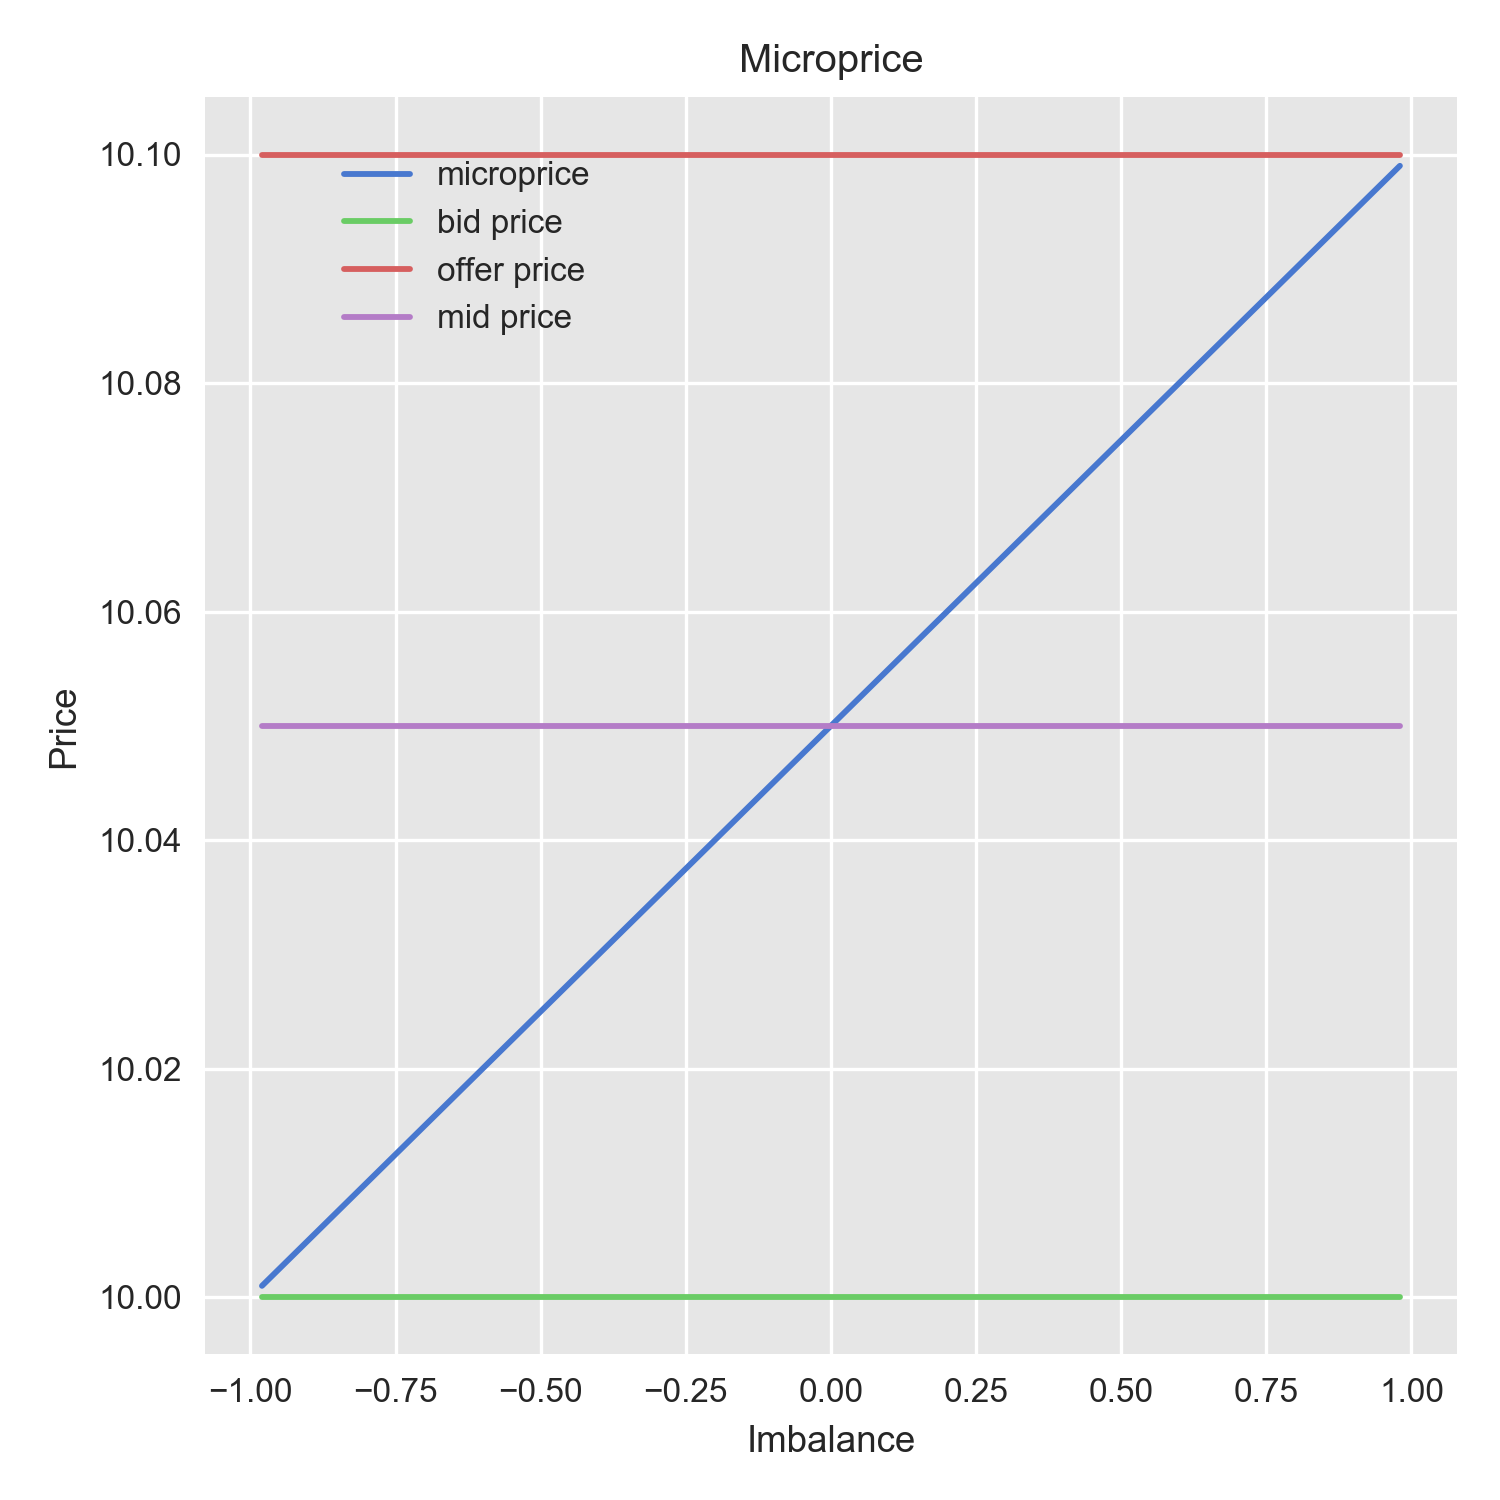
\includegraphics[width=0.75\textwidth]{chapters/chapter_trade_data_models/figures/microprice.png} 
		\caption{Microprice for different levels of imbalance. \label{fig:microprice}}
	\end{figure}

One can easily devise other measures of microprices that incorporate order book imbalance as well as the impact of the last traded price. \\


\noindent\textbf{Trade Imbalances:} For every trading transaction there is always one side that is the initiator of the trade, and in general the counterpart that runs out of patience that decides to pay the spread. This may be due to trading by an informed trader or by trader who has some urgency to trade. In either case an imbalance between the amount of buyer-initiated volume versus seller initiated volume would likely be instructive. One way to define trade imbalance is
	\begin{equation}\label{eq:vbs}
	\text{TI}=\frac{V_b}{V_b+V_a}.
	\end{equation} 
A zero-one trade imbalance would mean that all the volume was buyer (seller) initiated. 


While this metric is simple to use, the challenge is to categorize a trade as buyer or seller initiated. For most practitioners who do not have access to Level III data and only has data on quotes and trades this is not trivial as there is a limited amount of research around the efficacy of various algorithms. For Level III data, this information is available for lit venues. However, this is not the case for dark venues where the trade classification of large blocks could be quite valuable.


The most popular approach for trade classification was proposed by Lee and Ready 1991)~\cite{leeready} as mentioned in Chapter 6 with subsequent revisit on this topic by Chakraborty, B. and Moulton, P. C. and Shkilko, A. (2012)~\cite{chakrabarty2012short}. The simplest version of this algorithm goes like this:
        \begin{itemize}
        \item If the execution price is greater than the prevailing mid price the trade is taken as buyer initiated.
        \item If the execution price is less than the prevailing mid price the trade is classified as seller initiated.
        \item If the execution price is equal to the prevailing mid price the trade is marked the same way as the previous trade.
        \end{itemize}
As noted in Chakraborty et al. (2012)~\cite{chakrabarty2012short}, for short sales, the algorithm has proven only moderately predictive to 70\% accuracy using contemporary quotes and trades. This is due to various causes. One such cause is the asynchronous nature of the trade and quote streams and where a quote change could be time stamped slightly before the trade that affected it, leading to mis-classification. The classification improves if the quotes are lagged one second.



\section{Limit Order Book (LOB): Studying Its Dynamics}

Before we formally present the models, we want to provide a review of how the analysis of LOB data has been approached. Biais, Hillion and Spatt (1995)~\cite{spalt} study the trading activity in Paris Bourse (a fully automated limit order market), the dynamics of order flow and how the order flow varies with the state of the order book and marketplace events relevant to the asset. It is found that the conditional probability of a limit order placement is larger when the bid-ask spread is larger and when the order book is not deep. If a market order has been placed the chance that the next order posted provides liquidity is generally higher. The placement of orders also follows a pattern with new orders coming in the morning when the price discovery occurs and cancellations and large orders occur in the evenings. The durations between trades do indicate that the intensity of trade varies during the course of a day. The main tool used in these calculations is contingency table which provides both marginal and conditional probabilities. 


\subsection{LOB Construction and Key Descriptives}

It is important to be able to construct the order book from the Trades and Quotes data. We present here the example discussed in Cao, Hansch and Wang (2009)~\cite{caohanschwang} which is quite elegant. The buy and sell side orders are represented as step functions. 
        \begin{enumerate}[--]
        \item The height of the first step of the book is the mid-price. For step `$i$', $i=1,2,\ldots$, the height on the buy side is the difference in price, $p_i-p_{i-1}$. 
        \item The length of a step `$i$' is the aggregate number of shares, $Q_i$ at price `$p_i$'.
        \item Similar procedure is carried out in the sell side.
        \item To make the order book comparable for different stocks, heights are normalized by the price gap between tenth price and the mid-price. 
        \end{enumerate}

To illustrate we consider the same data used in Cao et al. (2009)~\cite{caohanschwang} (Table III) which is given below (partially):
	\begin{table}[!ht]
	\centering
	\caption{Descriptives of shape of LOB \label{tab:descLOB}}
	\begin{tabular}{rrrrr}
	& \multicolumn{2}{c}{Length (\%)} & \multicolumn{2}{c}{Height (\%)} \\
	Steps & Buy & Sell & buy & sell \\
	1 & 11.97 & 11.94 & 5.07 & 5.23 \\
	2 & 13.23 & 12.67 & 8.55 & 8.97 \\
	3 & 12.06 & 11.56 & 9.25 & 9.59 \\
	4 & 11.04 & 10.77 & 9.84 & 10.12 \\
	5 & 10.59 & 10.49 & 10.24 & 10.45 \\
	6 & 9.91 & 10.16 & 10.63 & 10.62 \\
	7 & 9.55 & 9.87 & 10.95 & 10.71 \\
	8 & 9.06 & 9.58 & 11.28 & 10.88 \\
	9 & 8.80 & 9.52 & 11.71 & 11.38 \\
	10 & 3.80 & 3.43 & 12.48 & 12.06
	\end{tabular}
	\end{table}

Figure~\ref{fig:presentshape} presents the shape of the limit order book. 
	\begin{figure}[H]
	\centering
	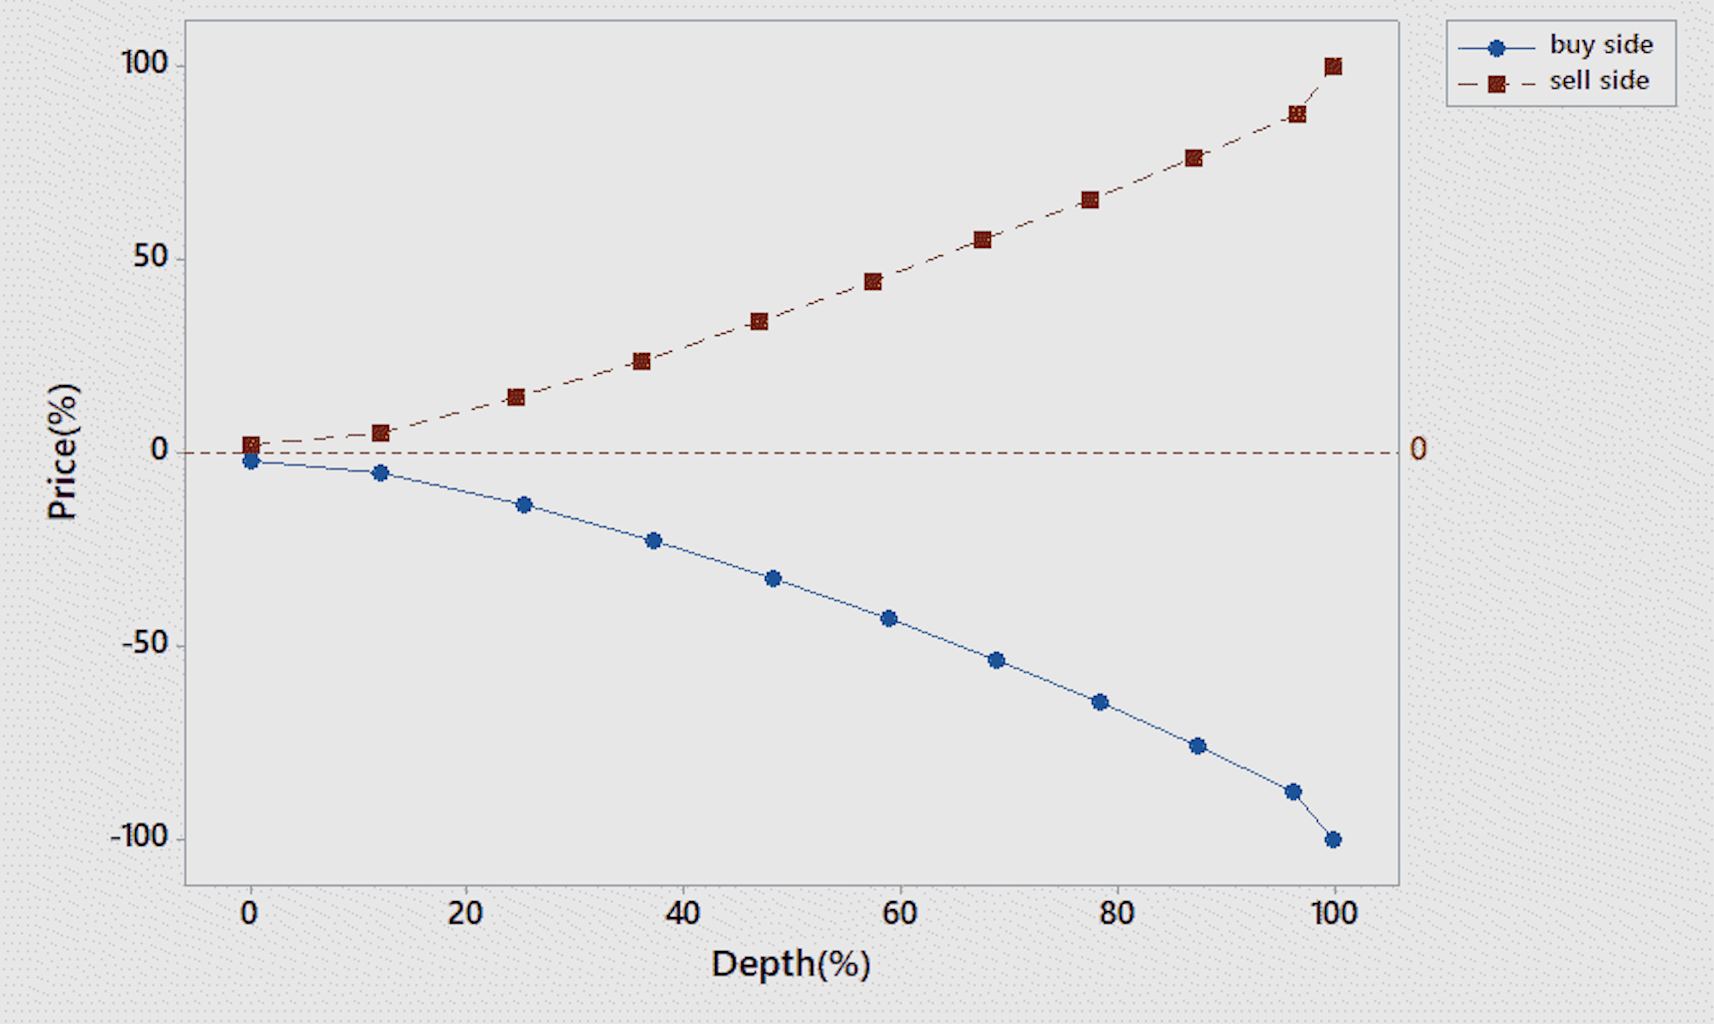
\includegraphics[width=1.0\textwidth]{chapters/chapter_trade_data_models/figures/lobshape.png} 
	\caption{The limit order book. \label{fig:presentshape}}
	\end{figure}


\noindent \textbf{Slope of LOB:} To begin with we can consider the slope of the order book both on the demand side and on the supply side using the quotes on both sides various depths (see Figure~\ref{fig:presentshape}). This provides information on order book imbalance that can be helpful for the trader to decide on the optimal time to enter or to exist the market (see Figure~\ref{fig:presentshape}). It is observed from Figure~\ref{fig:presentshape} that the bid-ask spread is at least twice the difference between quotes at successive depths. Thus the slope of the book is steeper closer to the best quotes. \\


\noindent\textbf{Order Flow:} The orders can be characterized as buyer or seller initiated and how aggressive they are. The aggressiveness is quantified by the size of the order. Most of the orders are small indicating that they could be part of a large parent orders. Both placement and cancellation of orders seem to decrease away from the best quotes. As the intra-day trading pattern follows typical diurnal pattern, both the depth and order flow must be adjusted for the time of the day. Some observations (stylized facts) worth noting are:
\begin{enumerate}[--]
\item Large (small) trades on one side of the market tend to be followed by large (small) trades on the same side. The same thing could be said about the new limit orders and cancellations as well. It is speculated that this may be due to traders reacting similarly to the same events or due to parent order splitting and automatic placement of child orders. \\

\item Cancellations on the buy side of the book are more frequent after market buy orders and the same for sell orders. This may be due to the fact that the large sell orders tend to convey negative information about the stock while the large buy orders convey positive information. Cancelations may also occur because of placement of some market orders are intended to probe the presence of any hidden orders. \\

\item Conditioning on the state of the book by size of bid-ask spread and the depth, it is observed that trades are more frequent when the spread is tight but the new orders inside the quotes are more frequent when the spread is large. The changes in spread are mainly due to liquidity shocks. \\

\item Frequency of trades tends to be clustered because competing traders who monitor the market closely are likely to place the orders when they read the market in their favor. It is observed that the trading activity is more intense with the information flow. Also observed are the following stylized facts: when the spread is large after liquidity shocks, traders place their orders quickly to take advantage of time priority. Thus the spread reveals back to original level. The expected time interval is generally lower after large trades than after other trades whether the spread is large or not.
\end{enumerate}


Thus the study by Biasis et al. (1995)~\cite{spalt} provides a set of concrete measures that could be used to study the dynamics of the limit order book. Now we will delve into model formulations. 


\subsection{Modeling LOB Dynamics}
\subsubsection{Review of Early Models}

We begin with one of the earlier models to appear in the econometric literature (Lo, MacKinlay and Zhang (2002)~\cite{maczhang}); they used the data from Investment Technology Group (ITG) that contained time stamped information on each limit order from submission to cancellation or execution. With three possible paths for each submitted order, the associated (a) time-to-cancellation/modification, (b) time-to-first fill and (c) time-to-completion are tracked and models are developed for each path on both sides of the order. Because ITG largely deals with the institutional investors, the results apply only to a limited segment of the traders. The modeling approach is to get the execution times as the first-passage time to the limit price assuming that price follows a geometric Brownian model with a drift:
	\begin{equation}\label{eqn:dp(t)}
	dP(t)= \alpha \cdot P(t) \; dt + \sigma \cdot P(t) \; dW(t),
	\end{equation}
where $W(t)$ is a standard Brownian motion. A buy limit order with a price `$P_l$' is executed in the time interval $[t_0,t_0+t]$ only if $P_{\text{min}} \leq P_l$ and the probability is
	\begin{equation}\label{eqn:expprob}
	P_r(P_{\text{min}} \leq P_l \;|\; P(t_0)=P_0)= 1- \left(1 - \left(\dfrac{P_l}{P_0}\right)^{2\mu/\sigma^2}\right) \Phi\left[\dfrac{\ln(P_0/P_l) + \mu t}{\sigma \sqrt{t}}\right],
	\end{equation}
where $\mu=\alpha - \frac{1}{2} \sigma^2$ and $\Phi(\cdot)$ is the cumulative distribution function of the standard normal. 


Note (\ref{eqn:expprob}) can be alternatively stated as, if `$T$' denotes the limit order execution time, $F(t)=P(T \leq t \;|\; P_0)$ for buy orders and similarly for sell orders, $F(t)=P_r(P_{\text{max}} \geq P_l)$. To see if the model is appropriate for the data at hand compare the theoretical c.d.f. of $F(t)$ to empirical c.d.f. using the well-known result that these are uniformly distributed. Fix `$\tau$' as the fixed sampling interval and with $r_t=\ln(P_t)-\ln(P_{t-1})$, the estimates of $\mu$ and $\sigma^2$ are:
	\begin{equation}\label{eqn:sampleestm}
	\hat{\mu}= \dfrac{1}{N\tau} \sum_{j=1}^N r_j, \quad \hat{\sigma}^2= \dfrac{1}{N} \sum_{j=1}^N \dfrac{(r_j - \hat{\mu} \tau)^2}{\tau}
	\end{equation}
where `$N$' is the number of observations in the sample. 


The above First Passage Time (FPT) model was used for filled orders without taking into account that there were other orders that were cancelled or were modified in that duration. The model's other limitations include not accounting for time priority, not including other relevant variables such as price volatility, spreads, etc.. The model's performance using the empirical cumulative distribution function is shown to be lacking. The model (\ref{eqn:expprob}) is expanded as
	\begin{equation}\label{eqn:cumexpmodel}
	F(t)=p_r(T_k \leq t \;|\; X_k,P_{lk}, S_k, I_k)
	\end{equation}
where $T_k$ is the execution of time of $k$ orders, $P_{lk}$ is the limit order price, $S_k$ is the size and $I_k$ is the side indicator. An alternative function, the hazard rate (briefly discussed in Chapter~2)
	\begin{equation}\label{eqn:hazard}
	h(t)=\dfrac{f(t)}{1-f(t)}= \dfrac{f(t)}{S(t)}
	\end{equation}
is found to be useful to operationalize and explain the modeling of survival rate of time-based events; Note $S(t)$ is called the survivor function. The censoring information ($\delta_i=1$ if observation `$i$' is censored) can be incorporated with $t_i$, $i$th realization of the random variable, $T$. It is assumed that the censoring mechanism is independent of the likelihood the limit order is executed. Using the generalized Gamma (defined in Chapter~2) as $f(t)$, the models are estimated.


The following variables are used as explaining variables:
        \begin{enumerate}[--]
        \item Distance between mid-quote and limit price.
        \item Prior trade indicator for buyer or seller initiated.
        \item Measures of liquidity.
        \item Measures of market depth.
        \item Measures that reflect change in trading activities. 
        \end{enumerate}
It is shown that this model does fare better than FPT model to capture the execution times. But an important limitation is ``\dots censoring as a result of prices moving away from the limit price would be a violation of the underlying assumption since prices at the time of censoring are not included in $X_i$.'' We show in our analysis of Level III data, a key determinant for cancellation of an order is that price moving away from the limit price that the trader has desired. \\


\noindent \textbf{Other Early Models:} There are a number of studies that have looked into order book dynamics using models that arise from Theory of Point Processes. Bouchard, Mezard and Polters (2002)~\cite{bouchardmezard} investigate the interaction between order flow and liquidity; it is observed that the distribution of incoming limit order prices follow a power law around the current price and the overall shape of the book in terms of volume on both sides is rather systematic. Smith, Farmer, Gillemot and Krishnamunthy (2003)~\cite{smithfarm} and Farmer, Gillemot, Lillo, Mike and Sen (2004)~\cite{farmermikesen} study how the order flow influences price formation; the price impact of market orders is a function of touch price depth and spread size. 


To have a more complete and realistic picture of how the LOB evolves, we must consider `hidden liquidity.' Almost all exchanges allow traders to hide all or portions of their orders. The so called, ``iceberg order'' is split into several smaller parts and is queued along with the other orders, but only the displayed quantity is visible and is part of the market depth. When the order reaches the front of the queue only the displayed is executed. Several reports could be as high as 26\%. In the models discussed below, we will not address the hidden liquidity issue, which will be taken up in a later section.


Modeling of LOB dynamics has drawn on ideas from economics, physics, statistics and psychology. The approach taken in economics literature is to focus on the behavior of the traders and the dynamics is modeled as sequential games (Rosu (2009)~\cite{irosu09}). Others, such as researchers from physics, have treated order flows as random and statistical mechanics techniques are used to study the dynamics. Other studies, such as Parlour and Seppi (2008)~\cite{parseppi} and Bouchaud et al. (2009)~\cite{bouchaud2009} are useful references for studies that come from economics point of view. We will review some models that are of recent origin. \\


\subsubsection{Recent Models}

\noindent\textbf{Cont, Stoikov and Talreja (2010)~\cite{contstoi}}: In this model of the limit order book, the number of limit orders at each price level in the book is taken to be a continuous-time Markov chain. The evolution of the order book through market orders, limit orders and cancellations is represented as a counting process. The model replicates the evolution of the events using independent Poisson processes. The study views LOB as a system of queues subject to order book events whose occurrences are modeled as a multidimensional point process. Before we state the specific questions and the models implications, we define certain useful quantities. 


It is taken that the price grid as $P(n)=\{1,2,\ldots,n\}$ multiples of a price tick. The number of outstanding orders in the book $|X_t^i|$ at price $i$, collectively, $X_t \equiv (X_t^1,\ldots,X_t^n)$ is taken to be continuous-time Markov chain; if $X_t^i<0$, then there are $-X_t^i$ bid orders at price `$i$' and if $X_t^i>0$, then there are $X_t^i$ ask orders at price $i$. Now we have,
	\begin{equation}\label{eqn:bestmidspread}
	\begin{split}
	\text{Best Ask Price: }& p_A(t)=\inf\{i \colon X_t^i>0\} \\
	\text{Best Bid Price: }& p_B(t)=\sup\{i \colon X_t^i<0\} \\
	\text{Mid Price: }& p_M(t)=(p_A(t)+p_B(t))/2 \\
	\text{Spread: }& p_S(t)=p_A(t)-p_B(t)
	\end{split}
	\end{equation}
The depth of the order book is stated relative to best bid and best ask on either side of the book. This way the model can be applied to order book for any equity subject to ever changing, best bid and best ask. Define
	\begin{flalign} \label{eqn:qaqb}
	&& Q_i^B(t)&= \begin{cases} X_{p_A(t)-i}(t), & 0<i<p_A(t) \\ 0, & p_A(t) \leq i <n \end{cases} && \notag \\
	\text{and} && \phantom{x} & \phantom{x} && \\
	&& Q_i^A(t)&= \begin{cases} X_{p_B(t)-i}(t), & 0<i<n-p_B(t) \\ 0, & n-p_B(t) \leq i <n \end{cases} && \notag
	\end{flalign}
Thus, $Q_i^B(t)$ and $Q_i^A(t)$ denote the number of buy orders at a distance `$i$' from ask and the number of sell orders at a distance `$i$' from bid, respectively. This representation highlights the shape (or depth) of the book relative to the best quotes on either side as in Figure~\ref{fig:presentshape}.


The following assumptions are made on the order arrivals: market buy or sell orders arrive at independent exponential times with rate, $\mu$. Limit buy or sell orders arrive at a distance of `$i$' ticks from the opposite best quote at independent exponential times with rate $\lambda(i)$. The cancellations of limit orders occur at a rate proportional to the number of outstanding orders, $\theta(i)X$. All these events are assumed to be mutually independent.


How the limit order is updated with the inflow of above events can be described as follows: for a state $x \in \mathbb{Z}^n$ and $1 \leq i \leq n$, let $x^{i \pm 1}=x \pm (0,\ldots,1,\ldots,0)$, where `1' denotes the change in the $i$th component. For example, a limit buy order at price level, $i<p_A(t)$ increases the quantity at level `$i$', from $x$ to $x^{i-1}$ with rate $\lambda(p_A(t)-i)$. Similarly, limit sell order arrived which changes the order book from $x$ to $x^{i+1}$ with rate $\lambda(i-p_B(t))$ for $i>p_B(t)$. For market buy order decreases at the ask price $i$ and hence $x \to x^{p_A(t)+1}$ with rate `$\mu$' and the sell order at the bid price, `$i$' will change the book status, $x \to x^{p_A(t)+1}$ with rate $\mu$. Cancellation of a buy order at price level, `$i$', will decrease the quantity at the rate $\theta(p_A(t)-i)|X_p|$ for $i<p_A(t)$ and the sell order will decrease the quantity at the rate of $\theta(i-p_B(t))|X_p|$ for $i>p_B(t)$.


It is assumed that the limit order arrival rate $\lambda(i)$ follows a power law
	\begin{equation}\label{eqn:powerlaw}
	\lambda(i)=\dfrac{\kappa}{i^\alpha}
	\end{equation}
which is confirmed by several empirical studies. The empirical estimates of the parameter are based on the following quantities: $s_m$ is the average size of the market orders, $s_l$ is the average size of the limit orders and $s_c$ is the average size of the cancelled orders. Also let $N_l(i)$ be the total number of limit orders that arrived at a distance `$i$' from the opposite best quote and $T_*$ is the total trading time in minutes and $N_m$ is the number of market orders during the same time. Then 
	\begin{equation}\label{eqn:hatlambdant}
	\hat{\lambda}(i)= \dfrac{N_l(i)}{T_*}, \quad 1 \leq i \leq 5
	\end{equation}
where $\hat{\lambda}(i)$ is extrapolated beyond five positions using the power law in (\ref{eqn:powerlaw}) simply by minimizing $\sum_{i=1}^5 (\hat{\lambda}(i)- \frac{\kappa}{i^\alpha})^2$, over `$\kappa$' and `$\alpha$'. The arrival rate is estimated as:
	\begin{equation}\label{eqn:hatnmt}
	\hat{\mu}=\dfrac{N_m}{T_*} \cdot \dfrac{s_m}{s_l}
	\end{equation}
The cancellation rate as noted earlier is defined as proportional to the number of order at that price level,
	\begin{equation}\label{eqn:hatthetacase}
	\hat{\theta}(i)=
	\begin{cases}
	\dfrac{N_l(i)}{T_*Q_i} \cdot \dfrac{s_c}{s_i}, & i \leq 5 \\
	\hat{\theta}(5), & i>5
	\end{cases}
	\end{equation}
It is understood that the cancellation is not due to executing market orders.


While these descriptives are easy to compute and are intuitive, but the main interest in modeling high frequency dynamics of order book is to predict short-term behavior of various key quantities that were identical earlier that may help in algorithmic trade executions. Some relevant questions are as stated before, given the state of the order book, what is the probability that mid-price will move up, what is the probability of executing both buy and sell order at the best quotes before the price changes etc.. These conditional probabilities are evaluated using Laplace transforms.


We present some key results in Cont et al. (2010)~\cite{contstoi}. These results generally make intuitive sense. The probability of queue going up when there are no orders in the queue, for $1 \leq d \leq 5$, given that the best quotes are not changing is
	\begin{equation}\label{eqn:queuecon}
	p_{\text{up}}^d(m)=
	\begin{cases}
	\dfrac{\hat{\lambda}(d)}{\hat{\theta}(d)m+\hat{\lambda}(d)+\hat{\mu}}, & d=1 \\
	\dfrac{\hat{\lambda}(d)}{\hat{\theta}(d)m+\hat{\lambda}(d)}, & d>1.
	\end{cases}
	\end{equation}
Other questions such as the probability that the mid price goes up when the spread $\geq 1$ etc. are based on the following quantities:
\begin{itemize}
\item Probability of a market buy order
	\begin{equation}\label{eqn:probmarketbuy}
	\dfrac{\mu^a}{\mu^b+\mu^a+\sum_j (\lambda_B(j)+\lambda_A(j)+\theta(j) Q_j^A(t)+\theta(j)Q_j^B(t))}
	\end{equation}
\item Probability of a limit buy order $d$ ticks away from the best ask
	\begin{equation}\label{eqn:problimitbuytick}
	\dfrac{\lambda_B(d)}{\mu^b+\mu^a+\sum_j(\lambda_B(j)+\lambda_A(j)+\theta(j)Q_j^A(t)+\theta(j)Q_j^B(t))}
	\end{equation}
\item Probability of a cancel buy order $d$ ticks away from the best ask
	\begin{equation}\label{eqn:probcanceltick}
	\dfrac{\theta(d)Q_d^B(t)}{\mu^b+\mu^a+\sum_j(\lambda_B(j)+\lambda_A(j)+\theta(j)Q_j^A(t)+\theta(j)Q_j^B(t))}
	\end{equation}
\end{itemize}
The model was evaluated using data sets from Tokyo Stock Exchange. The model is shown to capture realistic features of the order book profile.
	\begin{figure}[!ht]
   	\centering
   	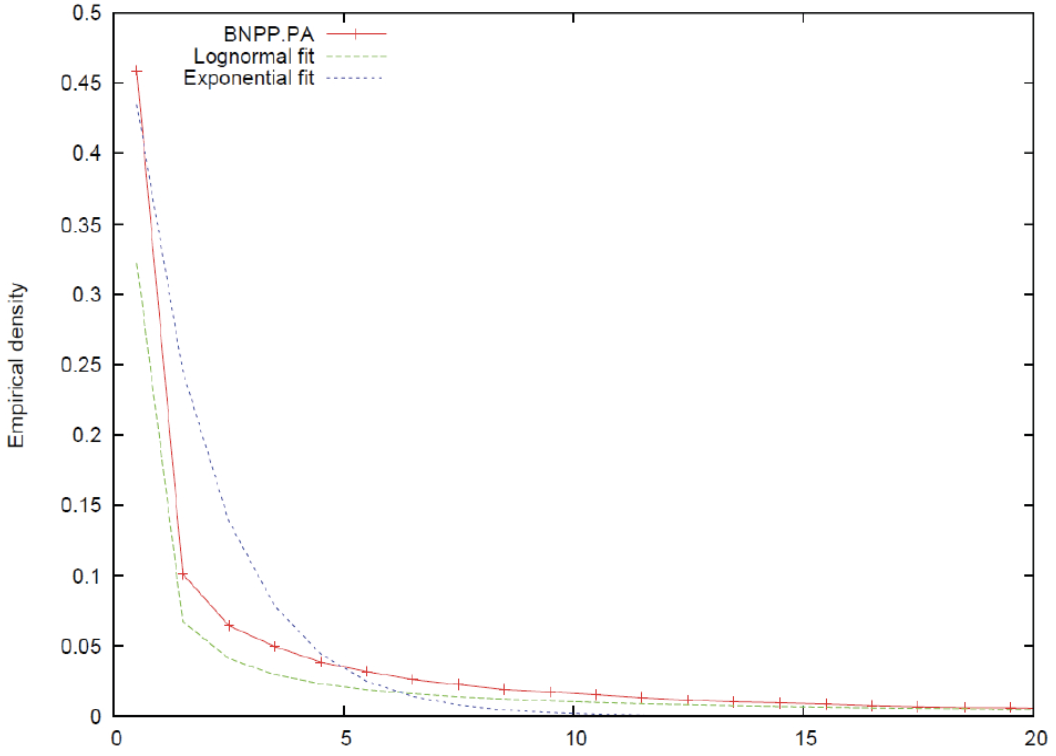
\includegraphics[width=0.9\textwidth]{chapters/chapter_trade_data_models/figures/intertime.png} 
   	\caption{Distribution of inter-arrival times of market orders for stock BNPP.PA (Chakraborti et al. 2011)~\cite{chaktokpat}. \label{fig:intertimefig}}
	\end{figure}

The use of Poisson processes to model the flows of limit orders, market orders and cancellations makes this method analytically tractable. The model captures the steady-state shape of the order book (although there may be other distributions that may be fit better besides Poisson, see Figure~\ref{fig:intertimefig}) but it may not be useful for predicting short-term behavior that may be more relevant for the traders. The assumption of Poisson process results in that the intensity of arrivals and cancellations that does not depend on the state of the order book which is somewhat unrealistic given the feedback loop relationship between the behavior of the market participants and the history of the order book. Recent works show that the memory-less property is not empirically valid. Orders tend to be clustered due to dependencies between liquidity taking and liquidity providing and also due to algorithmic execution of parent order that is split into numerous child orders. Also, the assumption that all orders are of the same size is too simplistic. 


Models based on marked point process are proposed when the mark represents order types, price, size etc.. The joint modeling assumes that the order flow is self-exciting, i.e. new orders or cancellations occur in an orderly point processes with an intensity function that depends on the history of the limit order book. These models are somewhat difficult to estimate and do not fully capture the empirical results such as volatility clustering etc.. \\


\noindent\textbf{Queue-Reactive Model:} Most of the market participants consider their target price with reference to market price, which depends on the order flows and the resulting changes in the state of the LOB. Huang, Lehalle and Rosenbaum (2015)~\cite{hlehros} study the LOB dynamics via a Markov queuing model when the market price remains constant and how the market price changes. The change in market price can occur when the execution occurs at the best price or a new order appears within the spread. This dual split of the model is termed as `queue-reactive model.' In the framework considered, three specific scenarios, where bid and ask sides are independent, independent except for the first two positions, on either side and where cross dependence between bid queue and ask queue is possible.


We will not delve into extensive details here, but briefly indicate the main gist of the model. Going for `$k$' positions on both sides of the order book, $X(t)= (q_{-k}(t),\ldots,q_{-1}(t),q_1(t),\ldots,q_k(t))$ is modeled as continuous time Markov jump process. The key quantities in the calculations are the intensity rates of arrivals of limit orders, cancellations and market orders. Under the independence assumption, the following behaviors are observed:

\begin{enumerate}[--]
\item Limit order arrival in the first position is approximately a constant function of queue size. At other positions away from the best positions, the intensity is a decreasing function of queue size. 

\item Intensity of order cancellation is an increasing concave function of $q_{\pm1}$, not linear as in Cont et al. (2010)~\cite{contstoi}; but after the first position, intensity is much lower as they are likely to move to the top of the book.

\item The rate of market order decreases exponentially with the available volume in the best positions. For the second position the shape of the intensity function is similar to the first position but the intensity decreases after that.
\end{enumerate}


In the case of dependency where bid side and ask side are correlated to each other, the above observations include the consideration of queue sites on the other side as well. In a paper with similar ideas, Abergel and Jedidi (2013)~\cite{aberjed} present a model that captures a stylized description of order book with the assumption of independent Poissonian arrival times. They also show that the price process converges to a Brownian motion. \\


\subsubsection{An Introduction: Hawkes Process}

Hawkes (1971)~\cite{hawkes71} introduced a model for self-exciting and mutually exciting point processes which capture the property that occurrence of an event increases the chance of further events occurring. Before we describe its applications in LOB modeling, we want to briefly discuss the main features of the model. If we let $\lambda(t)$ be the conditional intensity measured through the change in the number of events that occur in the time interval $(0,t)$ given the information available, then the self-exciting process has the intensity
	\begin{equation} \label{eq:seintensity}
	\lambda(t)= \mu + \int_0^t \gamma(t-u) \;dN(u)= \mu + \sum_{T_i<t} \gamma(t-T_i),
	\end{equation}
where $0<T_1<T_2<\cdots<T_n<\cdots$ are the times when events occur. When $\mu>0$ and $\gamma(u)=0$ provides a Poisson base level for the process. The function $\gamma(u) \geq 0$ is called the exciting kernel. Each event will increase the intensity and then will decrease until the next event occurs again when the intensity will go up. Some of the kernels suggested in the literature are:
	\begin{equation} \label{eq:suggex}
	\begin{split}
	\text{Exponential kernel: }& \gamma(u)= \alpha \cdot \beta \cdot e^{-\beta u} \quad\quad \mu>0 \\
	\text{Powerlaw kernel: }& \gamma(u)= \dfrac{\alpha \beta}{(1+\beta u)^{1+p}}
	\end{split}
	\end{equation}
Here `$\alpha$' represents the overall strength of excitation and `$\beta$' controls the relaxation time. 


Hawkes (2018)~\cite{hawkes18} provides a review of Hawkes processes in financial applications. Two extensions that are found to be useful are: one related to marked point processes, where associated marks with the event can trigger the excitement and the second relates to the processes when there are different types of events and how they can influence each other:
	\begin{equation} \label{eq:markedhawk}
	\begin{split}
	\text{Marked Hawkes Process: }& \eta(\lambda_t)= \mu(t) + \sum_{T_i<t} \gamma(t-T_i, \xi_i) \quad \quad T_i<t \\
	\text{Mutually Exciting Process: }& \lambda_{i,t}= \mu_i + \sum_{j=1}^D \sum_{T_{j:r}<t} \gamma_{ij} (t- T_{j:r}).
	\end{split}
	\end{equation}
Here `$\xi_i$' are marks such as `volume' and `$D$' is the different types of events with their own point processes. 


\noindent\textbf{Models for Volatility Clustering:} The features of volatility clustering and the significant autocorrelations in durations between order arrivals and significant cross-correlation of arrival rates across various event types are better captured by multi-dimensional Hawkes process. For a given $M$-dimensional point process, let $N_t=(N_t^1,\ldots,N_t^M)$ denote the associated counting process and the Hawkes process is characterized by intensities, $\lambda^m(t), m=1,\ldots,M$ as
	\begin{equation}\label{eqn:lambdamdoub}
	\begin{split}
	\lambda^m(t)&= \lambda_0^m(t) + \sum_{n=1}^M \int_0^t \sum_{j=1}^P \alpha_j^{mn} e^{-\beta_j^{mn}(t-s)} dN_s^n \\
	&=\lambda_0(t) + \sum_{n=1}^M \sum_{t_j<t} \sum_{j=1}^P \alpha_j^{mn} e^{-\beta_j^{mn}(t_j -t_i^n)}
	\end{split}
	\end{equation}
where the number of exponential kernels, $P$, is fixed and $t_i^n$ is the $i$th jumping time of the $m$th variate. The scale and decay parameters, $\alpha^{mn}$ and $\beta^{mn}$ express the influence of the past events $t_i^n$ of type `$n$'. The baseline model in (\ref{eqn:lambdamdoub}) does not incorporate the effect of bid-ask spread on order flow. It is shown in the literature that $\alpha$ and $\beta$ parameters do depend on the bid-ask spread. A simulated Hawkes process (Toke 2011~\cite{toke}) is given in Figure~\ref{fig:hawkes}. As noted earlier, the main characteristic of the Hawkes process is that intensity goes up at each event and decays exponentially between events. 
	\begin{figure}[!ht]
   	\centering
   	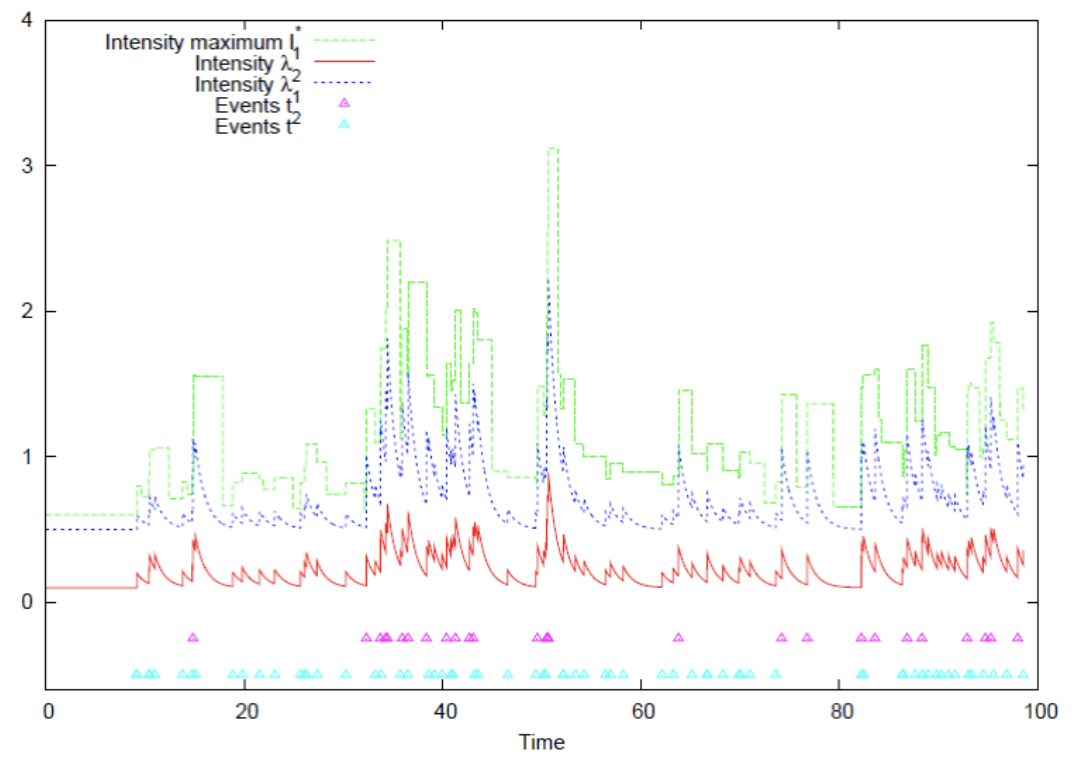
\includegraphics[width=0.9\textwidth]{chapters/chapter_trade_data_models/figures/hawkes.png} 
   	\caption{Simulated two-dimensional Hawkes process. \label{fig:hawkes}}
	\end{figure}


The evolution of the order book is driven by six different intensity functions, but the model changes with the value of the spread. The base intensity and the decay rates are all assumed to be functions of the spread. The model is quite complex and requires the estimation of a large number of parameters, which in turn requires vast amount of data for calibration. 


We will briefly discuss the likelihood estimates of the model in (\ref{eqn:lambdamdoub}). First, we want to observe for a Poisson process, the intensity function $\lambda(t)=\lambda_0$, a constant. The log-likelihood of the model,
	\begin{equation}\label{eqn:loglikemod}
	\ln \mathcal{L}(\{t_i\}_{i=1,2,\ldots,N}) = \sum_{m=1}^M \ln \mathcal{L}^m(\{t_i\}),
	\end{equation}
where
	\[
	\ln \mathcal{L}^m(\{t_i\})= T - \sum_{i=1}^N \sum_{n=1}^M \dfrac{\alpha^{mn}}{\beta^{mn}} (1- e^{-\beta^{mn}(T-t_i)}) + \sum_{t_i^m} \ln[ \lambda_0^m(t_i^m) + \sum_{n=1}^M \alpha^{mn} R^{mn}(l) ]
	\]
and 
	\[
	R^{mn}(l)= \sum_{t_\kappa^n t_l^m} e^{-\beta^{mn}(t_l^m-t_\kappa^n)}
	\]
is the cumulative decay function. Using the Multiplicative Random Time Change Theorem that states that with a certain transformation of the variables, the Hawkes process can be changed to a unit rate homogeneous Poisson process. Transforming the time variable `$t$' into `$\mathcal{T}$', where
	\begin{equation}\label{eqn:calt}
	\mathcal{T}= \int_0^t \lambda(s) \; ds
	\end{equation}
Hawkes process becomes a Poisson process with unit rate. Thus
	\begin{equation}\label{eqn:diffcalt}
	\mathcal{T}_i - \mathcal{T}_{i-1}= \Lambda(t_{i-1},t_i) = \int_{t_{i-1}}^{t_i} \lambda(s) \; ds
	\end{equation}
is exponentially distributed. 


More generally in the `$M$' dimensional multivariate case,
	\[
	\begin{split}
	\Lambda^m(t_{i-1}^m,t_i^m)&= \int_{t_{i-1}^m}^{t_i^m} \lambda_0^m(s) \; ds + \int_{t_{i-1}^m}^{t_i^m} \sum_{n=1}^M \sum_{t^n<t_{i-1}^m} \alpha^{mn} e^{-\beta^{mn}(s-t^n)} \; ds \\
	&+ \int_{t_{i-1}^m}^{t_i^m} \sum_{n=1}^M \sum_{t_{i-1}^m<t^n<s} \alpha^{mn} e^{-\beta^{mn}(s-t^n)} \; ds
	\end{split}
	\]
will follow exponential distribution. The $\Lambda^m(t_{i-1}^m,t_i^m)$ are known as compensators and can be verified empirically if they follow exponential distribution. \\


\noindent\textbf{Application of a Hawkes process:} We want to illustrate the model with an application. We first look at the statistical properties of the data and then look at the results of fitting one and two dimensional Hawkes processes to it. Our findings show that a two dimensional model based on Hawkes processes performs considerably better than a model based on two independent Poisson Processes. This provides strong evidence of the fact that the two key features of Hawkes processes (path dependency of the order flow and the possibility of modeling the interaction between the dimensions) are capable of capturing and replicating some of the key features of the empirical data. Moreover, there is evidence of significant and asymmetric interplay between the buy and the sell sides for the Limit Orders and evidence of limited interplay between the two sides when it comes to Market Orders. Finally, a study of the statistical properties of the orders showed a complex of alternating symmetric and asymmetric behavior of the LOB. 


The INET data for XOM (Exxon Mobil) for the 1st of September 2010 is used here. Figure~\ref{fig:freqsubmitarrivals} shows the submission frequency plot and we can see how in the first hour a half and in the last half an hour of the trading day there is a much higher submission frequency (with peaks of 25/30 orders submitted per second) than during the rest of the day (around 5--10 orders per second).
	\begin{figure}[!ht]
   	\centering
   	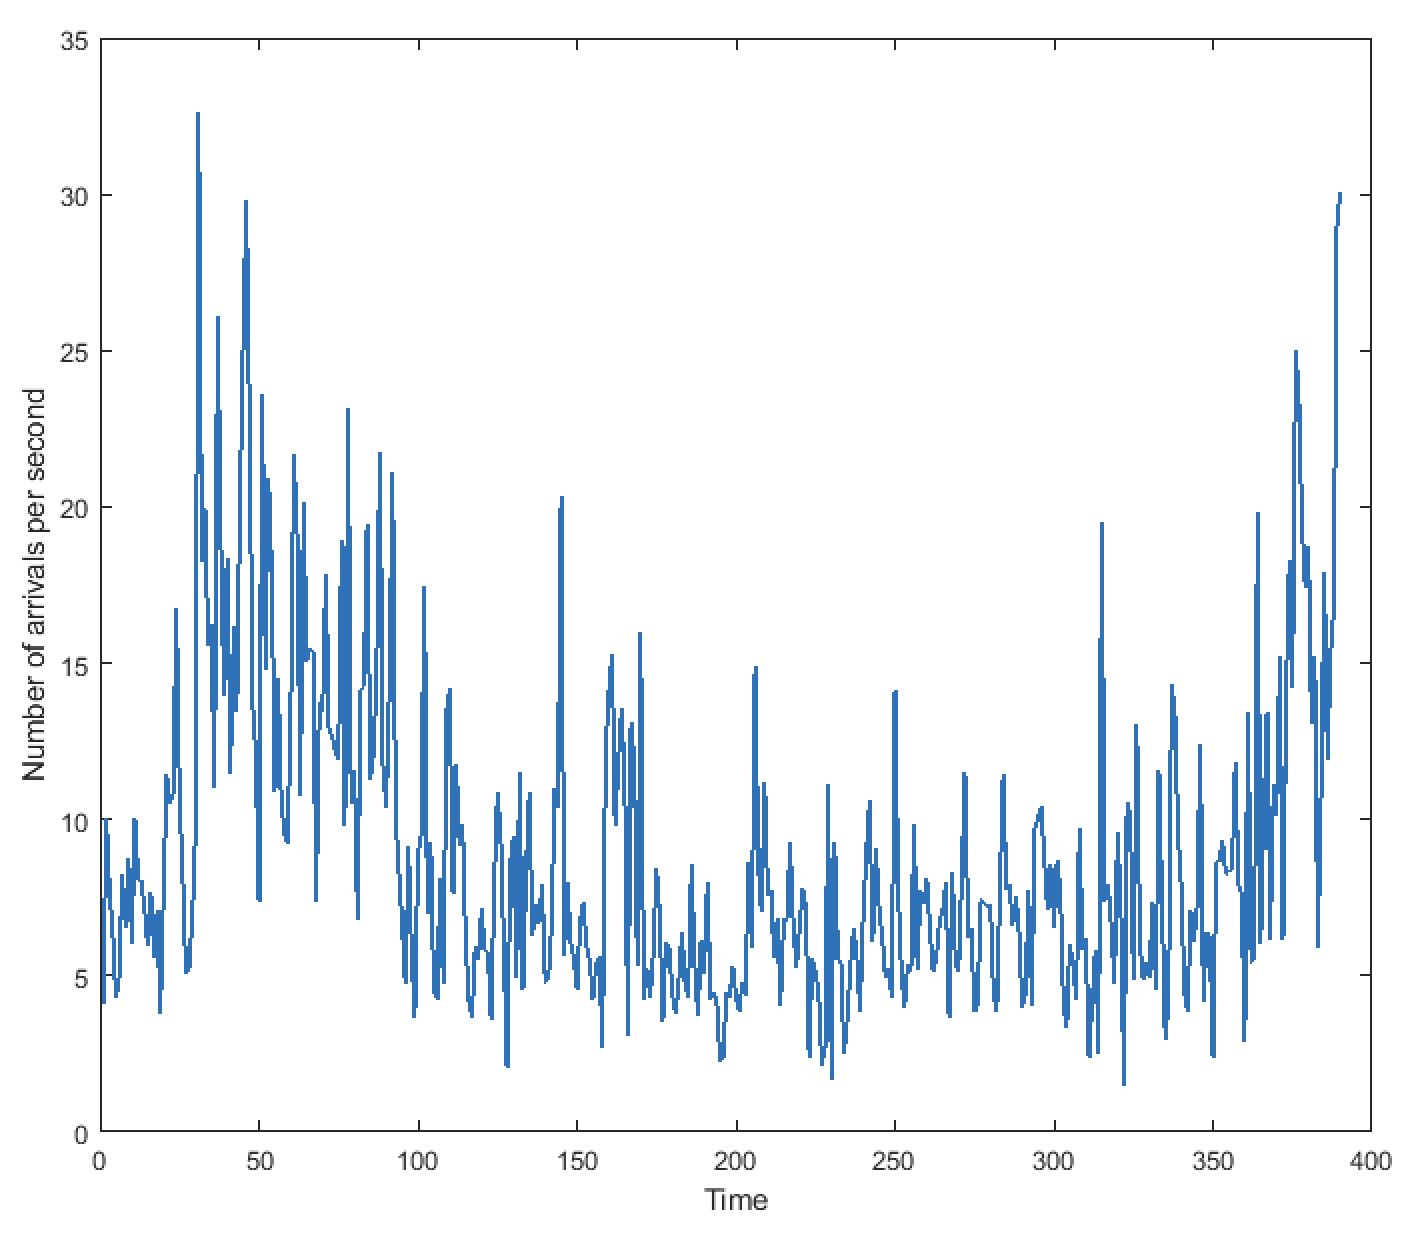
\includegraphics[width=0.75\textwidth]{chapters/chapter_trade_data_models/figures/freqsubmit.png} 
   	\caption{Frequency of Limit Order submission for 09/01/2010 (time in minutes after market opening). \label{fig:freqsubmitarrivals}}
	\end{figure}


This means that if we choose to look at the Limit Order flow with a model that doesn't allow for a varying baseline intensity, we will have to drop these two periods of increased trading activity and keep the data for only the middle portion of 6 hours of the trading day.


We then look at the data for the central portion of 6 hours of the trading day and find that market orders are just a fraction (4\%) of Limit Orders. Similarly, there is an imbalance in the side of the order submission (see Table~\ref{tab:xom}). 
	\begin{table}[htbp]
	\centering
	\caption{XOM data for 09/01/2010 \label{tab:xom}}
	\begin{tabular}{llll} 
	& Limit Orders & Market Orders & Total \\ \hline
	Buy & 48,541 & 2,107 & 50,648 \\ 
	Sell & 41,194 & 1,882 & 43,076 \\
	Total & 89,735 & 3,989 & 93,724
	\end{tabular}
	\end{table}
This shows how, on this trading day, most of the ``action'' was occurring on the Buy Side of the book which could mean that the markets were confident in an increase of the price of XOM (in line with the historical performance of the stock for that day).


The next step was to re-construct the Limit Order book from the order flow so to look at the life of the Limit Orders after their submission. From Table~\ref{tab:LOexec}, only about 6.5\% of all submitted LOs get at least partially filled with the percentage dropping to only about 6\% for those LO that actually get completely executed. Also, out of the LO that are completely filled nearly 90\% of them is filled in just one execution. This allows us to say that the magnitude of the LOs is comparable to that of the Market Orders, given that nearly all of them require only one Market Order to fill it completely. 
	\begin{table}[htbp]
	\centering
	\caption{LO executions and percentage breakdown by number of fills required \label{tab:LOexec}}
	\begin{tabular}{cccc}
	Number of LO & \% at least partially fill & \% completed in one fill & \% completely fill \\
	89, 735 & 6.57 & 5.35 & 6.15
	\end{tabular}
	\begin{tabular}{ccccccc}
	1 & 2 & 3 & 4 & 5 & 6 & $\geq$ 7 \\ \hline
	87.14 & 10.83 & 1.34 & 0.37 & 0.13 & 0.06 & 0.13
	\end{tabular}
	\end{table}


It can be observed that very few LO are actually submitted close to the market (hence have a chance to get executed) or that many of them don't stay in the book long enough to get executed. This led us to look into the life-time of the LOs and results are given in Table~\ref{tab:meanlo}.
	\begin{table}[htbp]
	\centering
	\caption{Mean LO cancellation and execution times (in seconds) \label{tab:meanlo}}
	\begin{tabular}{cccc}
	\multicolumn{2}{c}{No Fills} & \multicolumn{2}{c}{Partial Filles} \\ \hline
	Buy Orders & Sell Orders & Buy Orders & Sell Orders \\ \hline
	177.8 & 250.5 & 46.1 & 63.0 \\ \hline
	\multicolumn{2}{c}{First Fill} & \multicolumn{2}{c}{Completion} \\ \hline
	 25.3 & 56.2 & 25.6 & 57.6
	\end{tabular}
	\end{table}
In this particular case, LOs stay in the book for much longer if they are on the sell side than if they are on the buy side. This life-time difference for LOs on the two opposite sides of the book is consistent with what we saw earlier in the imbalance of the LO and MO submission. In fact, in this case as well we see how the buy side appears to be the more active side of the book. The shorter execution times for the orders on the buy side could be caused by either more aggressive pricing or by the price movements of the markets while the shorter lifespans and the higher number of orders on that side seem to indicate the use of more active trading strategies. However, there is another interesting observation that can be made. We see that on average a sell LO that is filled for the first time (but that doesn't get completely filled), is cancelled after about 7 seconds, compared to the 20 seconds that it would take had the order been on the buy side. This means that on average it takes three times longer for a partially (and never completely) filled order to be cancelled if it is on the buy side (which is the more active side) that if it is on the sell side (which is the less reactive side). The asymmetry between buy and sell side at the aggregated level has been noted in the literature.


The next step was to observe changes in the behavior of the book when moving further away from the market. We looked into the order submission and cancellation frequencies as a function of distance from the market price. Figure~\ref{fig:canfreq} and Figure~\ref{fig:freqsubmit1} show that most LO are submitted and cancelled at the market (respectively, 40\% and almost 30\%) and that the rates drop sharply with each price level further away from it. This supports the conclusion that the very small percentage of executed LO is not caused by the fact that most LO are submitted far away from the market and hence don't get the chance to get executed. We can also see how approximately 70\% (96\%) of all Limit Orders is placed in the top 5 (20) levels of the book and that 69\% (96\%) of all cancellations also occurs in the top 5 (20) levels. This a first indication of the fact that Level III data offers more information than Level II since with the top 5 levels of the book we were only able to capture around 70\% of all the occurring events. However, this also indicates that there is no need to use all the information provided in Level III data since by looking at only the top 20 levels of the book we are still able to capture nearly all of the occurring events. Both plots show a very similar behavior for the buy and sell side which led us to assume an almost symmetric behavior of the book. This assumption was later tested and confirmed at a 99\% confidence level with a two-sided Kolmogorov-Smirnov Test. 
	\begin{figure}[!ht]
   	\centering
   	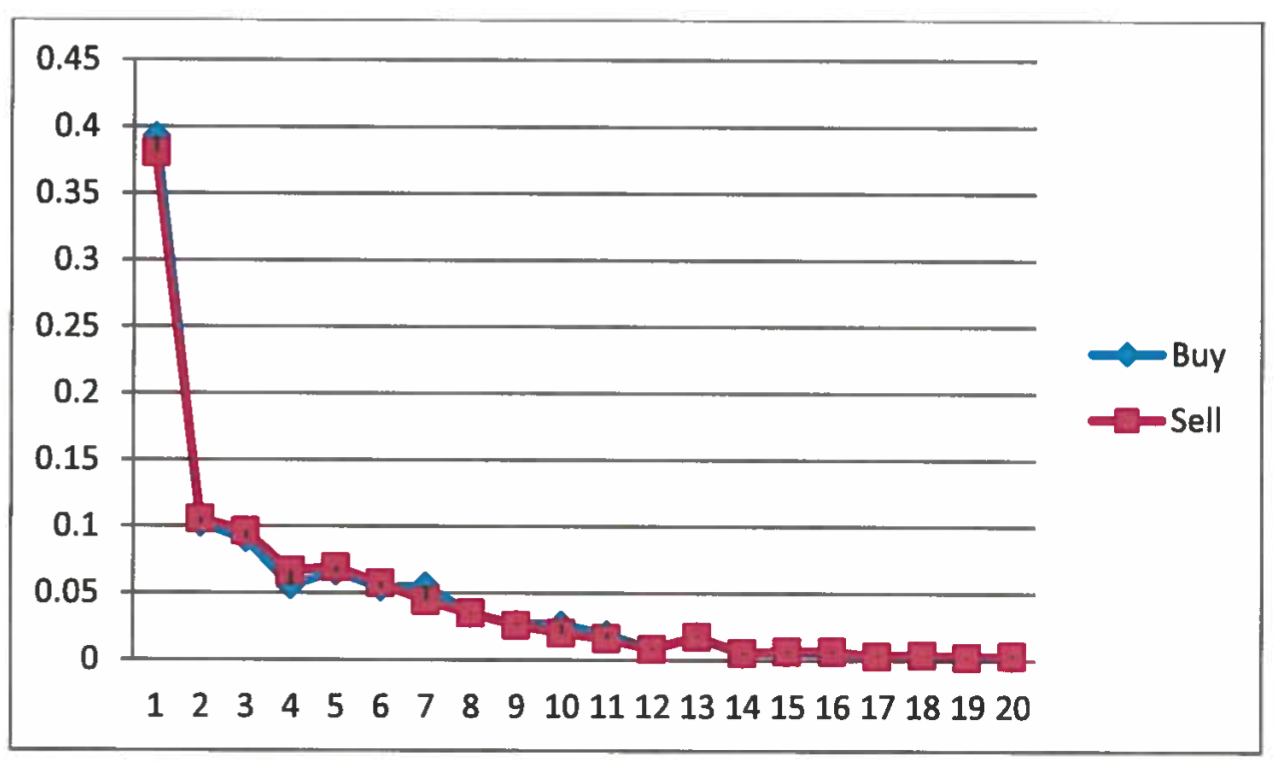
\includegraphics[width=0.75\textwidth]{chapters/chapter_trade_data_models/figures/subfreqnear.png} 
   	\caption{Submission frequencies--Distance near touch price \\ Kolmogorov-Smirnov Test Statistics$=0.61 \to$ fail to reject null at 1\% sig. level \label{fig:subfreqnear}}
	\end{figure}
	\begin{figure}[!ht]
   	\centering
   	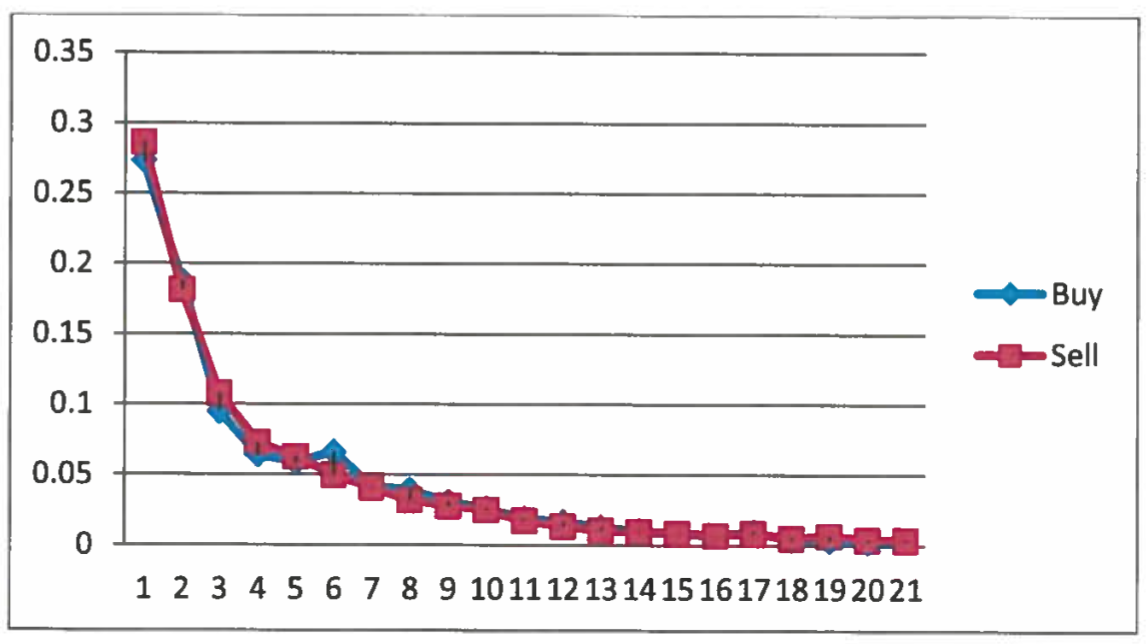
\includegraphics[width=0.75\textwidth]{chapters/chapter_trade_data_models/figures/canfreqnear.png} 
   	\caption{Cancellation Frequencies--Distance from near touch price \\ Kolmogorov-Smirnov Test Statistic$=0.83\to$ fail to reject null at 1\% sig. level \label{fig:canfreqnear}}
	\end{figure}


Better understanding what happens to the LOs once they enter the book is key in developing a more accurate way of choosing when to submit a LO or a MO. For this reason we also looked at the cancellation frequencies as a function of position in the queue and we found that (Figure~\ref{fig:canfreq}) most of the cancellations occur when the LO are in 4th or 5th position in the queue. In this case as well, we carried out a test of the assumption of a symmetric behavior of the book which confirmed previous similar findings. However, it would be more interesting to look at the cancellation frequencies as a function of overall distance from the market (as a measure of distance from possible execution). 
	\begin{figure}[!ht]
   	\centering
   	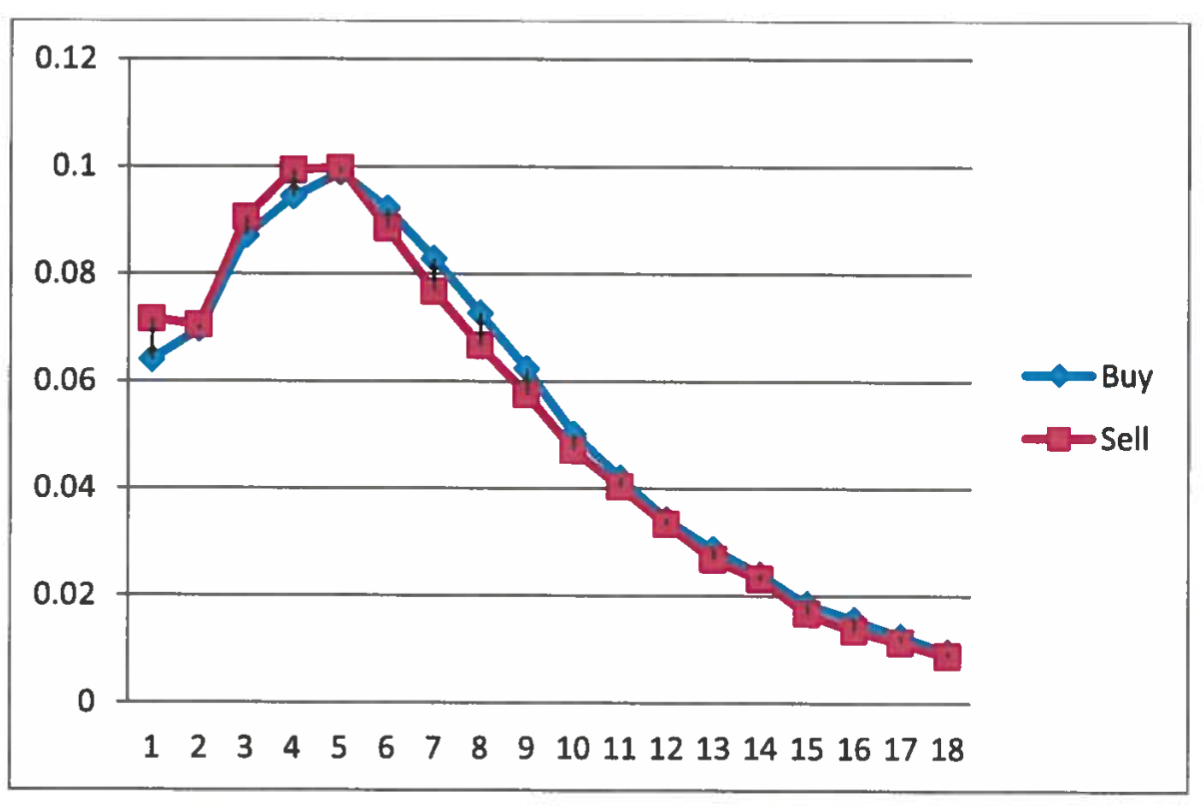
\includegraphics[width=0.75\textwidth]{chapters/chapter_trade_data_models/figures/canfreq.png} 
   	\caption{Cancellation Frequencies---position in queue. \label{fig:canfreq}}
	\end{figure}


With two more trading days (3rd and 9th of September 2013) data available, we are able to study the robustness of the above results. The submission and cancellation frequencies as a function of relative price which were symmetric for the 1st of September were not symmetric anymore on the 3rd of September. In this trading day, Figure~\ref{fig:freqsubmit1}, the peak of activity on the buy side occurred 12 price levels away from the market. This seems to suggest that on the 3rd of September the markets were betting that the price of XOM would drop in the foreseeable future, possibly reacting to some new event. A closer investigation of that time period revealed in the previous days the announcement by Exxon Mobil of the plan of closing a refinery which then led to a drop in the price shortly after 09/03/2010.
	\begin{figure}[!ht]
   	\centering
   	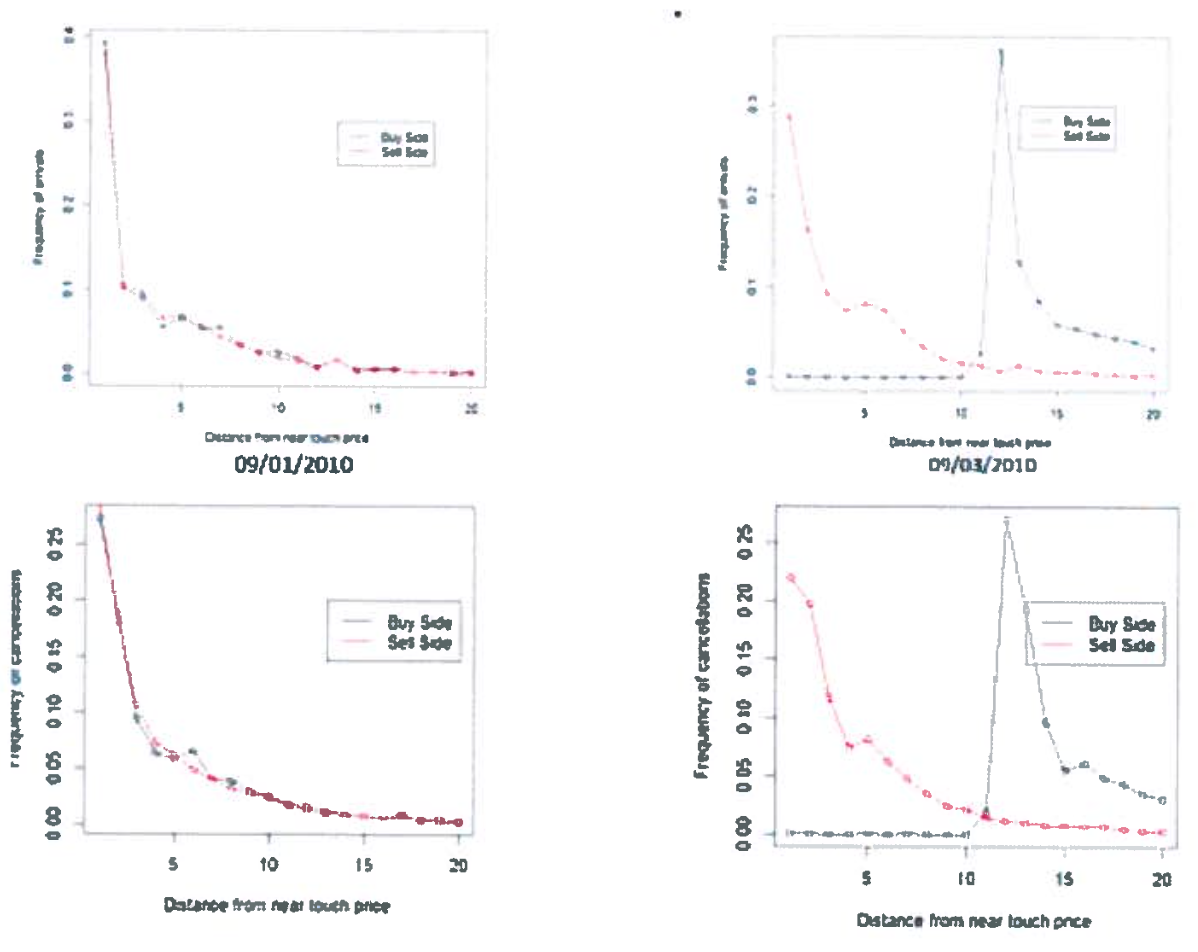
\includegraphics[width=0.75\textwidth]{chapters/chapter_trade_data_models/figures/losubcanfreq.png} 
   	\caption{LO submission and cancellation frequencies. \label{fig:losubcanfreq}}
	\end{figure}


A second interesting difference was in the amount of volume on the two sides of the book (Figure~\ref{fig:losubcanfreq}). Across the three days there was a significant volume imbalance with considerably more volume on the sell side than on the buy side but the amount of imbalance between the two sides changes significantly across the three days. Overall there is no explanation as to why there would be such a strong volume imbalance in favor of the sell side other than some kind of temporary anomaly. These findings seem to point out the fact that the shape and behavior of the LOB change dramatically across different days and that, in order to capture a more general/average behavior of the book, many more days of data are required. 
	\begin{figure}[!ht]
   	\centering
   	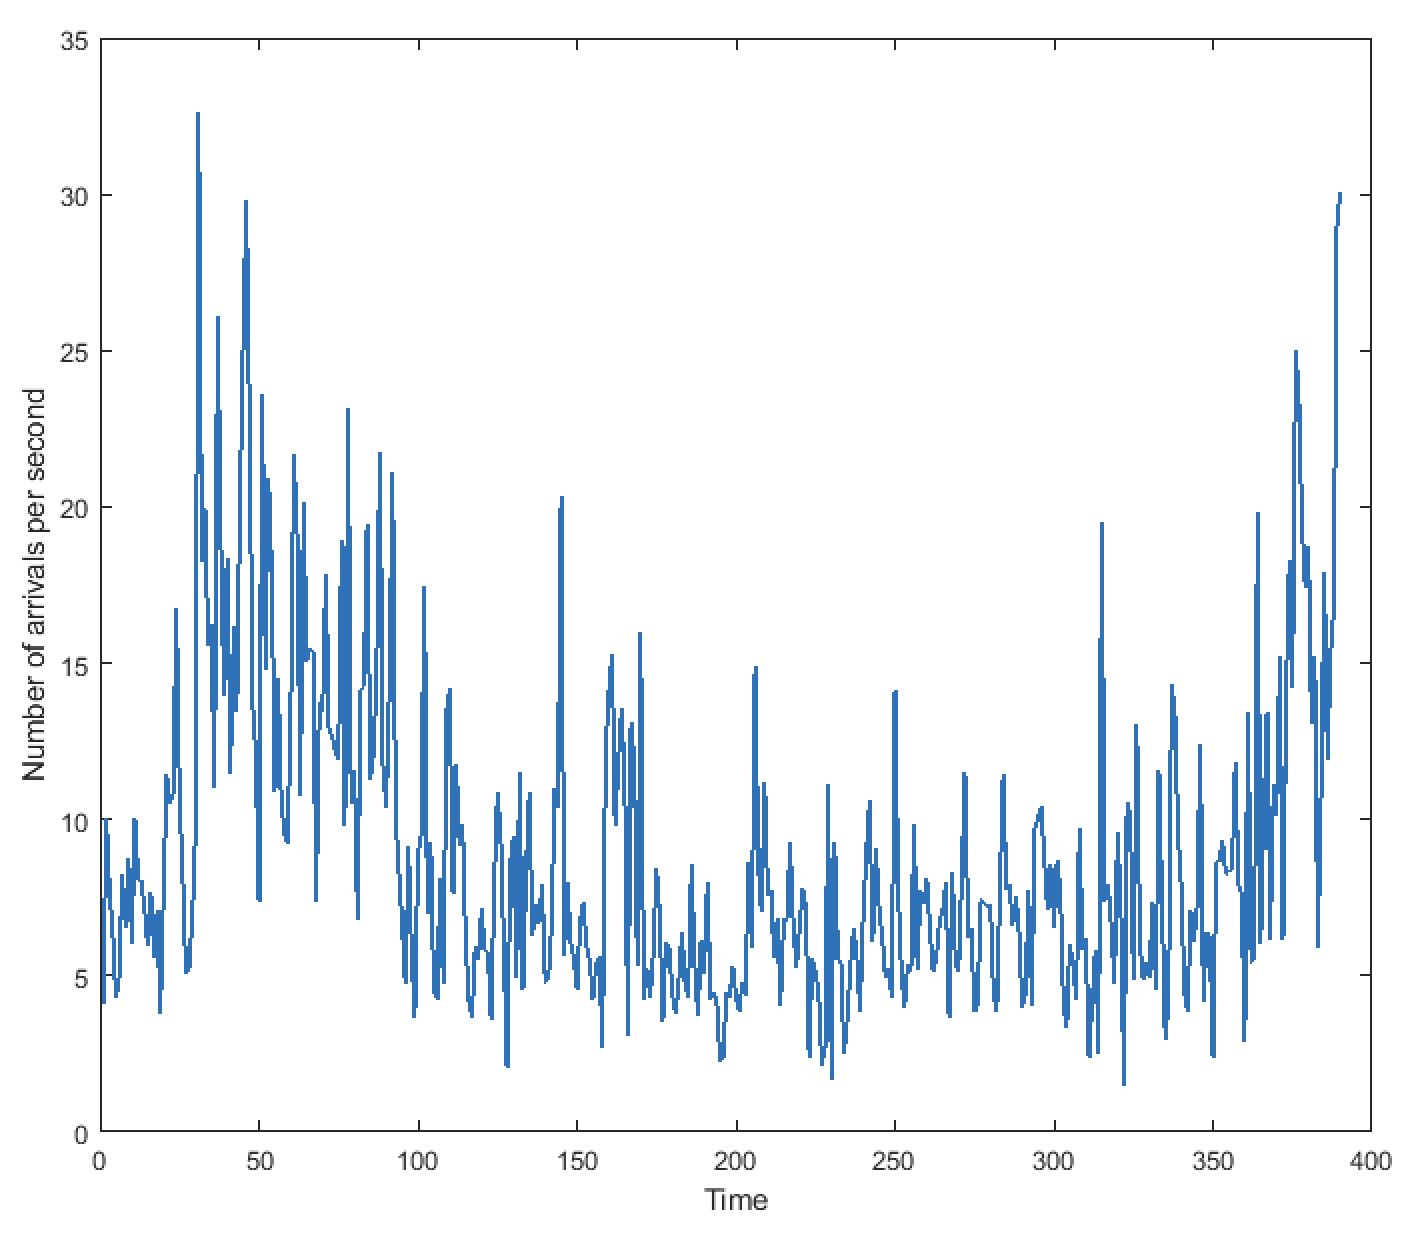
\includegraphics[width=0.75\textwidth]{chapters/chapter_trade_data_models/figures/freqsubmit.png} 
   	\caption{Frequency of Limit Order submission for 09/01/2010 (time in minutes after market opening). \label{fig:freqsubmit1}}
	\end{figure}
	\begin{figure}
	\centering
	\begin{subfigure}
	  \centering
	  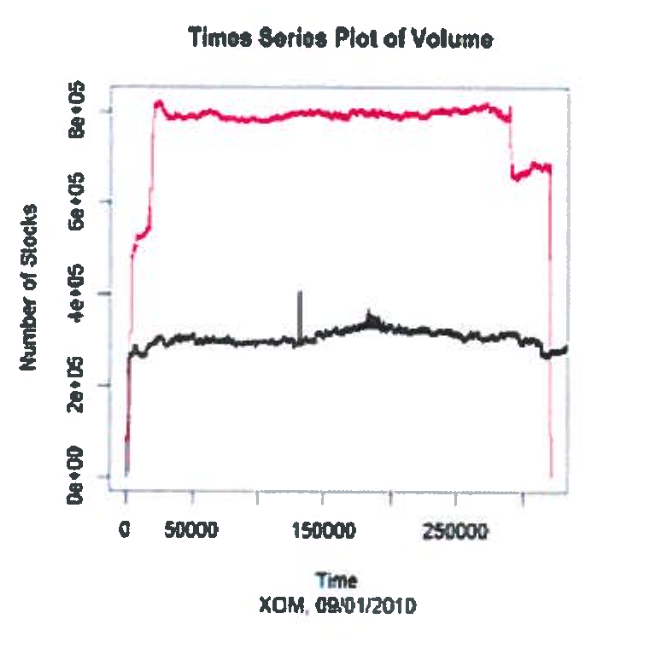
\includegraphics[width=.4\linewidth]{chapters/chapter_trade_data_models/figures/timevol1.png}
	\end{subfigure}%
	\begin{subfigure}
	  \centering
	  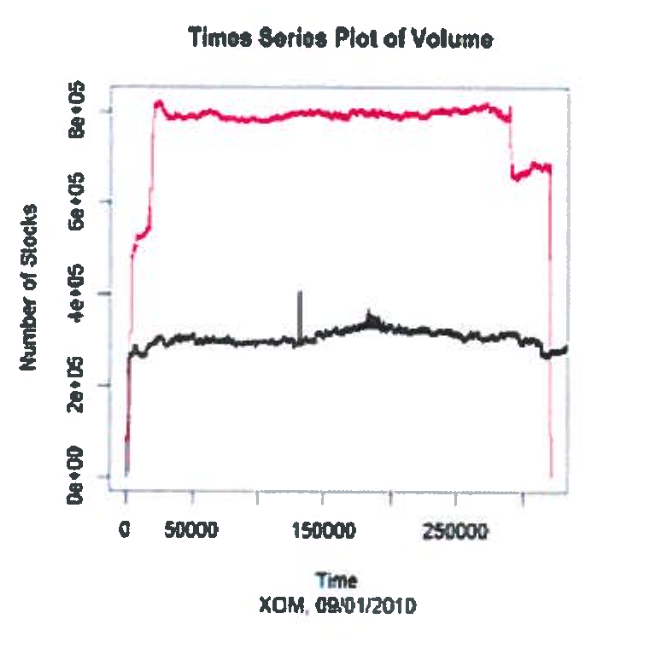
\includegraphics[width=.4\linewidth]{chapters/chapter_trade_data_models/figures/timevol1.png}
	\end{subfigure}
	\caption{Frequency of Limit Order submission for 09/01/2010 (time in minutes after market opening). \label{fig:freqsubmit2}}
	\end{figure}


\subsubsection{One-Dimensional Models}


We begin with a one dimensional model for the Limit Orders submitted on the buy side and one for those submitted on the sell side. Similarly, we build a one dimensional model for the Market Orders submitted on each side of the book. In the one dimensional case, the intensity function driving the Hawkes process is of the form
	\begin{equation}\label{eqn:lambda6}
	\lambda(t)= \lambda_0 + \alpha \sum_{t_i<t} e^{-\beta(t-t_i)}
	\end{equation}
with $\lambda_0$ indicating the baseline intensity, $\alpha$ indicating the jump in the intensity after the occurrence of an event and $\beta$ indicating the rate of exponential decay of the intensity after the occurrence of an event.


Table~\ref{tab:limmodbuy} and Table~\ref{tab:limmodsell} show the results of the MLE estimation of the parameters of the one dimensional models for the Limit Orders on the two sides of the book. The difference in the values of the estimates of the parameters for the two sides of the book (strongest on the 9th and weakest on the 1st of September) indicates that there is a level of asymmetry between these two sides. Also, even though the magnitude of the values of the parameters is the same for all three days (on each side of the book) there is still some variation between them, especially when we look at the model for the buy side. This seems to suggest that the behavior of the book can change considerably from day to day and that a considerable amount of data might be necessary in order to capture some kind of general behavior. 
	\begin{table}
	\centering
	\caption{1-D Limit Order Model (buy side) \label{tab:limmodbuy}}
	\begin{tabular}{c|ccc} 
		& $\lambda$ & $\alpha$  & $\beta$ \\ \hline
	09/01/2010 & 0.008108431 & 1.421767060 & 1.435094466 \\
	09/03/2010 & 0.006127003 & 1.290012415 & 1.299564704 \\
	09/09/2010 & 0.002341542 & 1.023410145 & 1.026757239
	\end{tabular}
	\end{table}
	\begin{table}
	\centering
	\caption{1-D Limit Order Model (sell side) \label{tab:limmodsell}}
	\begin{tabular}{c|ccc} 
		& $\lambda$ & $\alpha$ & $\beta$ \\
	09/01/2010 & 0.002055786 & 1.071071139 & 1.073989940 \\
	09/03/2010 & 0.002342963 & 0.983678355 & 0.986999404 \\
	09/09/2010 & 0.006123845 & 0.946420813 & 0.955774394
	\end{tabular}
	\end{table}


One of the advantages of having chosen an exponential decay for the intensity function of the process, becomes apparent when we analyze the meaning of these parameters. Using a well-known property of exponentially distributed variables, we can tell the half-life of the excitation effect caused by the occurrence of an event. In the specific, in our one-dimensional models we find that, on average, half of the excitation effect caused by the occurrence of an event is dissipated after about 0.7 seconds ($\frac{\ln 2}{\beta} \approx$ half-life). Also, the small estimated values for $\alpha$ indicate that the occurrence of an event has a very small impact on the likelihood of another event occurring. This seems to suggest that there is a weak self-excitation effect in the LO process when modeling it with a one-dimensional model. 


We then build, in a similar fashion, the two one-dimensional models for the flow of buy and sell Market Orders for all three days and obtained the following parameter estimation: 
	\begin{table}[!ht]
	\centering
	\caption{1-D Market Order Model (buy side) \label{tab:marketorderbuy}}
	\begin{tabular}{c|ccc} 
		& $\lambda$ & $\alpha$ & $\beta$ \\ \hline
	09/01/2010 & 0.0238743 & 7.3187478 & 19.8477514 \\
	09/03/2010 & 0.01450873 & 3.38168999 & 7.70581048 \\
	09/09/2010 & 0.0267254 & 4.8818834 & 13.5427254
	\end{tabular}
	\end{table}
	\begin{table}[!ht]
	\centering
	\caption{1-D Market Order Model (sell side) \label{fig:marketordersell}}
	\begin{tabular}{c|ccc} 
		& $\lambda$ & $\alpha$  & $\beta$ \\ \hline
	09/01/2010 & 0.02083999 & 9.38842281 & 24.55777564 \\
	09/03/2010 & 0.01616096 & 6.64370599 & 16.68090519 \\
	09/09/2010 & 0.0239992 & 8.2180945 & 25.0115980
	\end{tabular}
	\end{table}
The first thing that is obvious is the asymmetry between the buy and the sell sides. Nevertheless, for the Market Orders they asymmetry appears to be much more significant that it was for the Limit Orders, given the much bigger differences in the values of the estimated parameters. Also, for Market Orders we see that the occurrence of each event seems to have a much stronger impact on the likelihood of occurrence of future events than it was the case for Limit Orders. In fact, the values of $\alpha$ in Table~\ref{tab:marketorderbuy} and Table~\ref{fig:marketordersell} are considerably higher than those we saw in Table~\ref{tab:limmodbuy} and Table~\ref{tab:limmodsell}. Similarly, the values of $\beta$ are also much larger in the Market Order models than they were in the Limit Order models which means that the half-life of the excitation effect is much shorter for Market Orders (0.03 seconds vs. 0.7 seconds) than for Limit Orders. These differences in the results of the estimations are not that surprising if we consider what we saw in Table~\ref{tab:xom} for order submissions. Market Orders are submitted in much fewer numbers than Limit Orders which explains why even though the occurrence, such self-excitation has a very short lifetime. The significant increase in the chances of another Market Order occurring given that one has just occurred (even through for a very short time), might seem contradicting the fact that very few Market Orders actually occur. However, what can be inferred is that Market Orders depend strongly from the occurrence of other Market Orders and that they tend to cluster around submissions. 


\subsubsection{An extension}


An important limitation of this basic Hawkes Process model is that each event has the same impact on the intensity function. This implies that each event carries the same amount of information in the process. However, it is easy to imagine that a large LO would carry much more information about future price changes than a small one and this should be accounted for in the model. We include order size in the intensity function by scaling the size of the jump $\alpha$ in the value of the intensity by the ratio $\frac{w_i}{\overline{w}_l}$, where $w_i$ is the size of the LO and $\overline{w}_l$ is the average LO size up to that point. The intensity function for this ``extended'' one-dimensional model becomes
	\[
	\lambda(t)= \lambda_0 + \alpha \sum_{t_i<t} \dfrac{w_i}{\overline{w}_l} e^{-\beta(t-t_i)}
	\]
We then compared the performance of this ``size-adjusted'' model with the ``basic'' one by using the before mentioned \emph{Multivariate Random Time Chance} Theorem and looking at the Q-Q plot of the compensators for the two models. Figure~\ref{fig:lobuysideadj} and Figure~\ref{fig:losellsideadj} show how in both case (buy and sell Limit Orders) adjusting for size doesn't improve the fit of the model. This result is somewhat counter-intuitive given that more than 70\% of all Limit Orders are of size 100 shares and that this should imply that any deviation from this size explanation is that trading strategies are successful in concealing the true intension of the traders and that there is no significant information left in the size of the LO once that the strategies are implemented and the orders are submitted. 
	\begin{figure}[!ht]
   	\centering
   	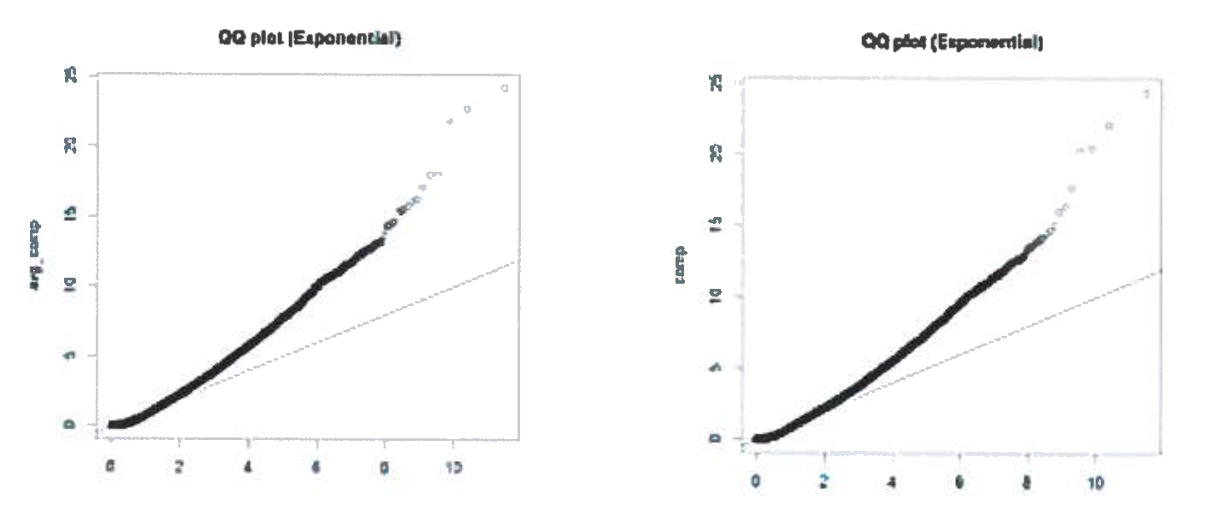
\includegraphics[width=0.75\textwidth]{chapters/chapter_trade_data_models/figures/lobuysideadj.png} 
   	\caption{LO--buy side with size adjustment and without. \label{fig:lobuysideadj}}
	\end{figure}
	\begin{figure}[!ht]
   	\centering
   	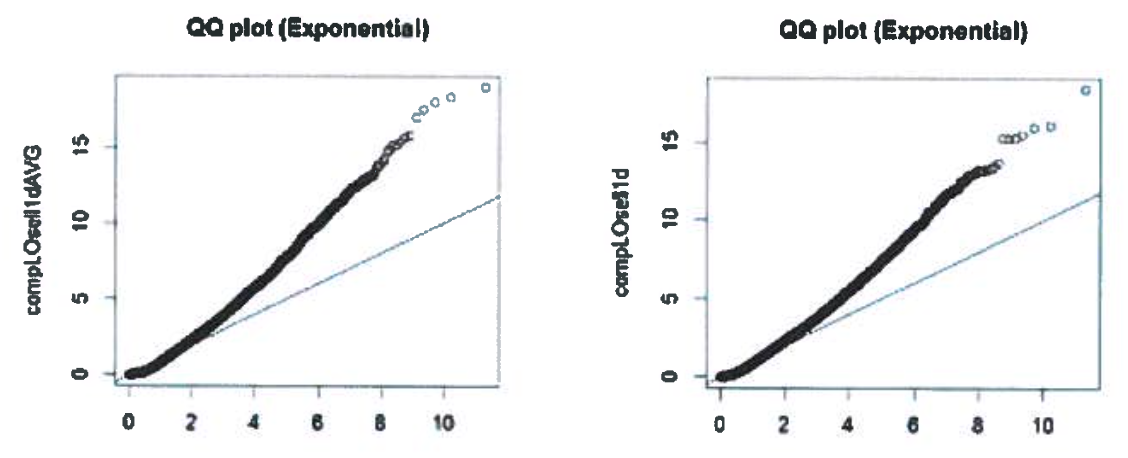
\includegraphics[width=0.75\textwidth]{chapters/chapter_trade_data_models/figures/losellsideadj.png} 
   	\caption{LO--sell side with size adjustment and without. \label{fig:losellsideadj}}
	\end{figure}


\subsubsection{Two-Dimensional models}


Our next step was to build two-dimensional models that would simultaneously model the buy and sell sides of the book and with two separate (yet interacting) intensity functions. The intensity functions for this kind of model become
	\[
	\begin{split}
	\lambda^B(t)&= \lambda_0^B + \int_0^t \alpha^{BB} e^{-\beta^{BB}(t-u)} \;dN_u^B + \int_0^t \alpha^{BB} e^{-\beta^{BS}(t-u)} \;dN_u^S \\
	\lambda^S(t)&= \lambda_0^S + \int_0^t \alpha^{SB} e^{-\beta^{SB}(t-u)} \; dN_u^B + \int_0^t \alpha^{SS} e^{-\beta^{SS}(t-u)} \;dN_i^S
	\end{split}
	\]
and we have 5 parameters for each dimension of the model for a total of 10 parameters across the two dimensions (buy and sell). The two additional parameters in each dimension account for the cross-excitation effect between the two dimensions. In our case, $\alpha^{BS}$ tells us the increase in the likeliness of a LO occurring on the buy side after the occurrence of a LO on the sell side, while $\beta^{BS}$ tells us the rate of decay of the buy side intensity after the occurrence of a LO on the sell side (and vice-versa for $\alpha^{SB}$ and $\beta^{SB}$). We then used MLE to estimate the parameters of the model and we can make several remarks about the results (Table~\ref{tab:2dimlomodel}).
	\begin{table}
	\centering
	\caption{2-Dimensional LO model \label{tab:2dimlomodel}}
	\begin{tabular}{lllll}  
	$\lambda^B=2.480 \cdot 10^{-5}$ & $\alpha^{BB}=14.386$ & $\beta^{BB}=31.517$ & $\alpha^{BS}=0.303$ & $\beta^{BS}=0.464$ \\ \hline
	$\lambda^S=2.677 \cdot 10^{-5}$ & $\lambda^{SS}=15.657$ & $\beta^{SS}=37.299$ & $\alpha^{SB}=0.149$ & $\beta^{SB}=0.312$ \\ 
	\end{tabular}
	\end{table}
	
	
There appears to be some asymmetry in the cross-excitation effects with the occurrence of an event on the sell side having a stronger impact on the likeliness of occurrence of an event on the buy side rather than the other way round ($\alpha^{BS}>\alpha^{SB}$). On the other hand though, since $\beta^{BS}<\beta^{SB}$, the effect on the sell side of an occurrence on the buy side is more persistent than that of an event on the buy side on the sell side (2.22 seconds vs. 1.49 seconds).
	\begin{figure}[!ht]
   	\centering
   	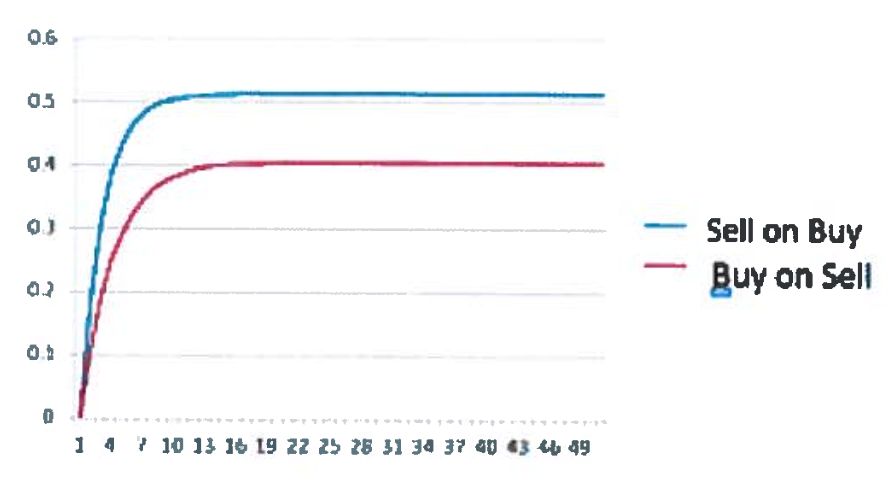
\includegraphics[width=0.75\textwidth]{chapters/chapter_trade_data_models/figures/asymcross.png} 
   	\caption{Asymmetry in cross-excitation effect. \label{fig:asymcross}}
	\end{figure}
The self-excitation components of the model are rather similar for both dimensions and it is interesting to point out the very short persistence of the self-excitation effect in both cases (about 0.02 seconds).


In order to evaluate whether the two key features of a model based on Hawkes processes (path dependency of the order flow and the possibility of modeling the relation between the various dimensions) are really helpful in improving the performance of the model, we decided to compare the performance of our model to that of a bi-dimensional model based on two independent Poisson Processes (which by definition of Poisson process does not account for any dependency in the order flow and by construction assume independence between the two dimensions). The results proved to be very encouraging with a remarkably better fit to the empirical data for the Hawkes Process based model (Figure~\ref{fig:4hawkes6}).
	\begin{figure}[!ht]
   	\centering
   	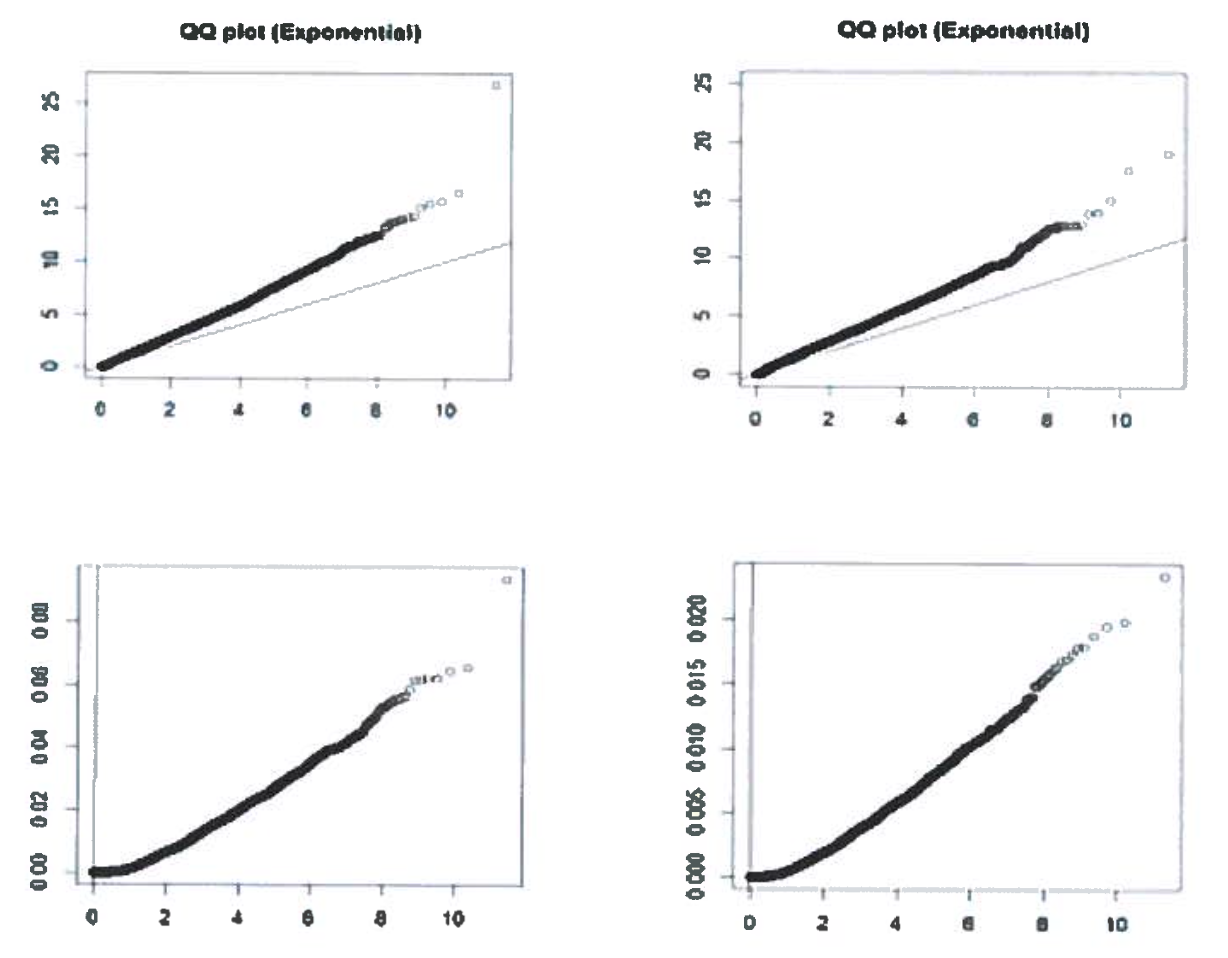
\includegraphics[width=0.75\textwidth]{chapters/chapter_trade_data_models/figures/4hawkes6.png} 
   	\caption{Top--Fit of Hawkes Process (buy \& sell); Bottom--Fit of Poisson Process (buy \& sell). \label{fig:4hawkes6}}
	\end{figure}


Following a similar procedure, we build a bi-dimensional model for the Market Orders and performed MLE to estimate the parameters. The results (Table~\ref{tab:2dimmomod}) showed very weak and symmetric cross-excitation between the dimensions which, however, turns out to be very persistent (141 seconds for the half-life of the effect of buy on sell and 215 seconds for that of sell on buy). The self-excitation effect is comparable across the two dimensions and is also very short lived (with a half-life of about 0.02 seconds).
	\begin{table}
	\centering
	\caption{2-Dimensional MO model \label{tab:2dimmomod}}
	\begin{tabular}{lllll}  
	$\lambda^B=2.701 \cdot 10^{-5}$ & $\alpha^{BB}=11.793$ & $\beta^{BB}=36.153$ & $\alpha^{BS}=0.0037$ & $\beta^{BS}=0.0049$ \\
	$\lambda^S=3.451 \cdot 10^{-5}$ & $\alpha^{SS}=12.454$ & $\beta^{SS}=35.063$ & $\alpha^{SB}=0.0017$ & $\beta^{SB}=0.0032$
	\end{tabular}
	\end{table}
	

Finally, we compared the performance of our model to that of the bi-dimensional Poisson Process. Similarly to the LO case, the model at hand significantly outperforms the Poisson Process one for both dimensions. 
	\begin{figure}[!ht]
   	\centering
   	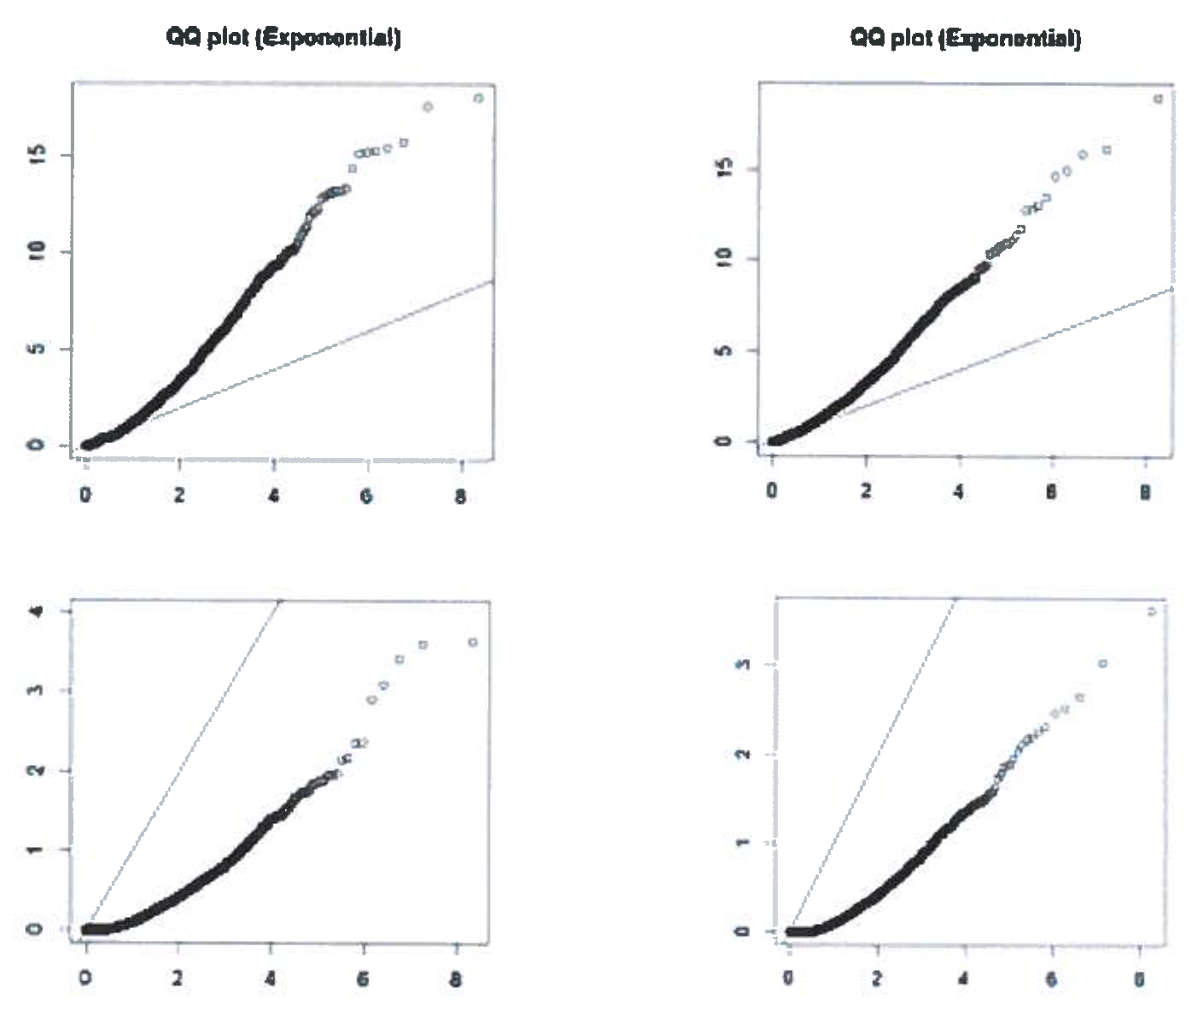
\includegraphics[width=0.75\textwidth]{chapters/chapter_trade_data_models/figures/4fig.png} 
   	\caption{Top--Fit of Hawkes Process (buy \& sell); Bottom--Fit of Poisson Process (buy \& sell). \label{fig:4fig6}}
	\end{figure}


\noindent\textbf{Limitations and findings:} There are some important considerations to be made from this analysis. The first issue is related to the cleaning of the data that was necessary in order to adapt it to our needs. In fact, Hawkes processes are ``simple'' processes which means that they don't allow for more events to occur simultaneously. Unfortunately, in the INET data it is quite common to encounter clusters of 10/20 events reported with the same timestamp. This is typical of high frequency data due to the approximation with which events are often reported and to the obvious limitation of the chosen time scale (e.g., milliseconds). In our case we decided to keep only the first event of each cluster, dropping all the others. A possible alternative used in the literature is to simply uniformly distribute the events from the clusters across the time interval given by the occurrence of the cluster and that of the next event. However, this approach could introduce bias in the parameter estimation phase. In fact, the clustering of events by itself is of interest.


Also, an important limitation of the bi-dimensional Hawkes Process model is that it is very computationally intense. Evaluating the five parameters for one of the two intensity function using data from only one trading day took almost two days. It becomes clear that in order to evaluate the parameters of a model using data for a longer time period of if evaluating the parameters for a model with higher dimension (hence with more parameters) will require considerably more computational power. 



\section{Models for Hidden Liquidity}

Investors have the option to place limit orders that are not visible to other traders but they are observable to exchange officials. These are called `hidden' or `iceberg' orders. The invisible order retains price but not time priority. It is possible to place a fraction of order visible but the rest hidden. When a visible portion gets executed, another fraction of the hidden order becomes visible. In NYSE, an order improving the quotes can be fully hidden. The posting of hidden orders is a second stage decision by the traders after choosing between market and limit orders. The risk of placing limit orders has been discussed earlier and an important element of that is the transparency or exposure risk that can signal to market participants the motive of the trader. This may result in other traders engaging in front-running strategies in anticipation of certain market movements. It is also speculated that orders are hidden when there is increased participation of informed traders and to minimize price impact when the execution probability is fairly high. 


De~Winne and D'Hondt (2007)~\cite{winne} study the choice between hidden and visible limit order placement via a logit model. The predictors include characteristics related to exposure and picking-off risks, such as order size relative to order book depth, the competitiveness of the price and the imbalance of the order book. Traders who monitor the order book closely can infer the presence of hidden orders and their depth by repeated posting on the opposite side. Using the detailed (more than level III) data from Euronext, orders are classified for their aggressiveness based on how much liquidity is taken out from the best opposite quote. It is observed that generally hidden orders are less aggressive than other limit orders. In modeling the data, because the exposure risk is larger toward the market close, the likelihood of more hidden orders at the near end of trading session is also taken into account and so is the trading intensity that varies during the day. 


The predictors of the models and the sign of estimated coefficients are listed below:
        \begin{enumerate}[--]
        \item Spread ($+$)
        \item order size as the ratio of depth on the same side and on the opposite side ($+$).
        \item Market imbalance based on best five visible quotes ($-$).
        \item Time left before the market close ($+$)
        \item Order aggressiveness measured by the five orders submitted prior to incoming order ($-$).
        \item Price aggressiveness, measured by the ratio of distance between the order price away from the best price on the same side and the price away from the opposite side's best price. ($-$)
        \end{enumerate}

It is concluded that the decision to hide and the order aggressiveness on the opposite side --- their relationship is ambiguous. All other estimates generally agree with what was postulated. When order aggressiveness is used as the response variable, it is shown that the traders adjust their order submissions when they see a signal of hidden order on the opposite side. Overall conclusion is that hidden orders are posted by not informed traders. 


Using the data from Spanish Stock Exchange, Pardo and Pascual (2012)~\cite{pardopas} study the market reaction to the presence of hidden orders discovered during the trading process. The high-frequency data reveals that traders in the opposite side become aggressive once they detect the hidden volume, but the price impact of hidden volume is purely temporary. It is not clear what the relevant information context is in the hidden orders.


To illustrate the presence of hidden orders, we consider the level III data whose description is given in Section~8.3.2.7 (Table~\ref{tab:level3data}). With this, we can construct the order book in real time (Figure~\ref{fig:limbk1}). For modeling some key elements considered are:
        \begin{enumerate}[--]
        \item The depth (in number of shares) at that price level after the order is submitted.
        \item The depth (in number of shares) at that price level before the order was submitted.
        \item The relative price (equal to 1 `at the market' and 2 at `1 price level away from market, etc.). 
        \end{enumerate}
        If the event is execution or cancellation,
        \begin{enumerate}[--]
        \item The distance in cents from opposite best price in the book.
        \item How long has the LO been in the book.
        \end{enumerate}
        Some that are common to all events (excluding Hidden Executions) are:
        \begin{enumerate}[--]
        \item If the Super Book (the market) is Locked, Crossed or OK.
        \item The relative spread.
        \item Number of shares at the Top of the book on that side.
        \item Number of shares at the Top of the book on the opposite side of the book.
        \item Number of shares at the Top 5 price levels of the book on that side.
        \item Number of shares at the Top 5 price levels of the book on the opposite side of the book.
        \item Weighted average price of the shares on the Top 5 levels of the book on that side.
        \item Weighted average price of the shares on the Top 5 levels of the book on the opposite side of the book.
        \item Relative spread of the weighted prices.
        \end{enumerate}
If the even is a hidden order execution:
        \begin{enumerate}[--]
        \item The price at which the Hidden Order is executed.
        \item The size of the executed Hidden Order.
        \item An indicator of what side is the trade; in fact, there is NO BUY or SELL indicator for hidden trades so I apply the Lee-Ready Rule. If it is a Buy, then `B'; if it is a Sell, then `S'; if it is at the midpoint, then `Na'.
        \item The distance in cents from opposite best price in the book.
        \end{enumerate}


For ease of presentation, we use CISCO data for a single day; CISCO stock is heavily traded and thus capture the typical intense market activity. To avoid the bias in results due to excessive trading activities around the opening and closing of the market, we consider only the duration between 9:35~AM to 3:55~PM, thus discarding data outside these time limits. Table~\ref{tab:distributionoforder} below provides how the orders submitted on both sides (Buy and Sell) are dealt with:
	\begin{table}[!ht]
	\centering
	\caption{Distribution of orders \label{tab:distributionoforder}}
	\begin{tabular}{l | ccc | r}
	& Buy & Midpoint & Sell & Total \\ \hline
	Cancelled & 166975 & --- & 175693 & 342648 (86.9\%) \\
	Executed (Visible) & 21041 & --- & 23595 & 44636 (11.3\%) \\
	Executed (Hidden) & 1702 & 3864 & 1394 & 6190 (1.8\%) \\ \hline
	Total & 189718 & 3814 & 200662 & 394194
	\end{tabular}
	\end{table}
It is clear a majority of orders gets cancelled with only 13\% of orders get executed. 


It is interesting to note that although only 13\% of the trades are hidden, they seem to occur and inter-dispersed through a trading day. The Figure~\ref{fig:priceplothidvis} indicates that the hidden ordrs are clearly embedded with the visible orders. Two useful observations follow from Table~\ref{tab:typeexc} below:
	\begin{table}[!ht]
	\centering
	\caption{Type of executed orders versus Side B (entries are median price and depth 1) \label{tab:typeexc}}
	\begin{tabular}{l | ccc| r}
	Type of Order & Buy & Na & Sell & Overall \\ \hline
	\multirow{2}{*}{Visibile} & 20.50 & --- & 20.51 & 20.50 \\
	& 39863 & --- & 39682 & 39800 \\
	\multirow{2}{*}{Hidden} & 20.50 & 20.52 & 20.54 & 20.51 \\
	& $-150$ & 50 & $-50$ & 50 \\ \hline
	\multirow{2}{*}{All} & 20.50 & 20.52 & 20.51 & 20.50 \\
	& 36047 & 50 & 36606 & 32765
	\end{tabular}
	\end{table}
The hidden orders are generally executed by orders placed closer to the top of the book and seem to result in better price.
	\begin{figure}[!ht]
	\centering
	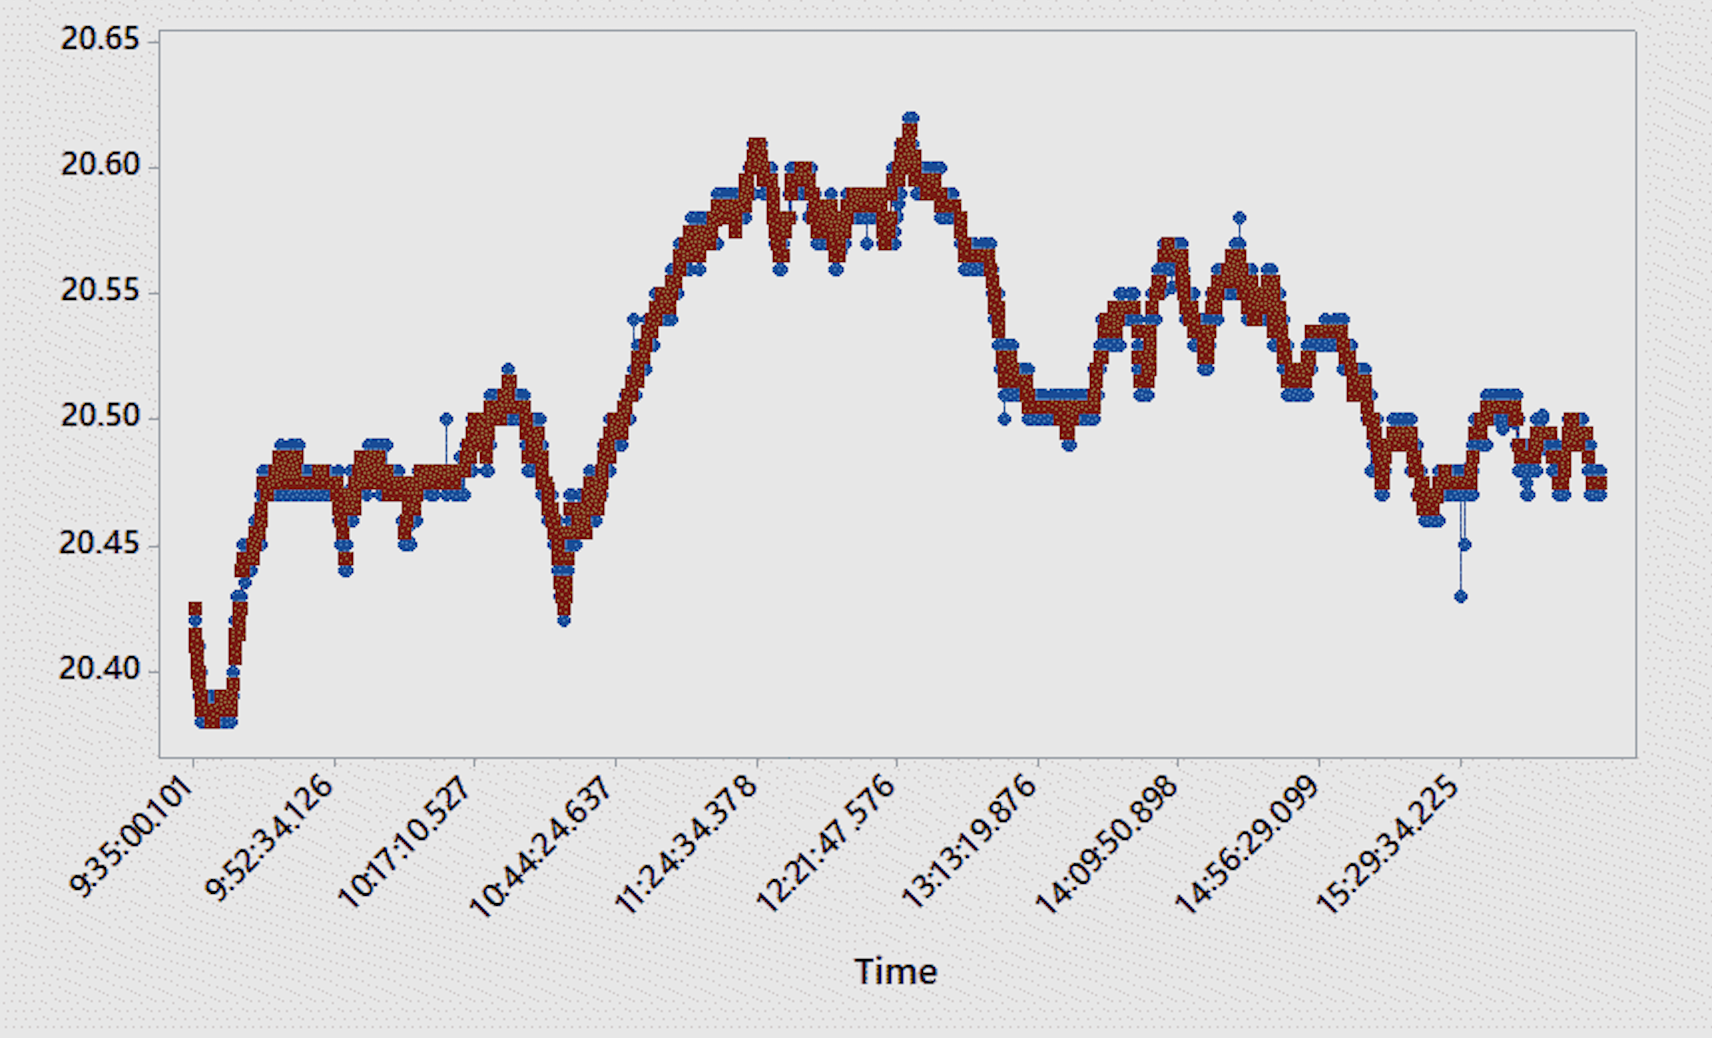
\includegraphics[width=1.0\textwidth]{chapters/chapter_trade_data_models/figures/priceplot.png}
	\caption{Price plot (Red: Hidden; Blue; Visible). \label{fig:priceplothidvis}}
	\end{figure}


Recent work by Bessembinder, Panayides and Venkataraman (2009)~\cite{bessenbinder} evaluates the strategies for order exposure using Euronext-Pairs Bourse data; the hypotheses are stated below:
\begin{enumerate}[--]
\item Order exposure increases execution probability and decreases time-to-completion.
\item Order exposure decreases execution probability and increases time-to-completion (supported).
\item Hidden orders are used primarily by (uninformed) traders to mitigate the option value of a standing limit order.
\item Hidden orders are used primarily by (informed) traders to protect themselves against defensive trading strategies (not true).
\item Hidden orders usage is more for larger orders, aggressively priced orders and when adverse selection risk is high.
\end{enumerate}
The discovery and estimation of hidden depth is of interest to traders; while discovery and this has been discussed in great detail in the context of dark pools, we want to comment on the existence and execution of hidden orders in the presence of a bast majority of visible orders. We study this via transition matrix; probability that the next trade is a hidden trade given that status of the current trade, whether it is visible or hidden:
	\begin{table}[!ht]
	\centering
	\caption{Transition Matrix \label{tab:transmatrix}}
	\begin{tabular}{c l | cc}
	& & \multicolumn{2}{c}{Current Trade} \\
	& & Visible & Hidden \\ \hline
	\multirow{2}{*}{Next Trade} & Visibile & 0.95 & 0.35 \\
	& Hidden & 0.05 & 0.65
	\end{tabular}
	\end{table}
This information along with depth information in Table~\ref{tab:transmatrix} indicate that hidden orders are executed somewhat together at the top of the book. 



\section{Modeling LOB: Some Concluding Thoughts}


With the availability of voluminous high-frequency data, there is as we saw in this chapter a considerable literature to understand the market micro-structure issues. The time-stamped data on each and every activity provides both opportunities and challenges. The challenge is in sorting out the signal from the noise. It gets even more complicated when we want to account for the activities over the time scale. The so-called Epps effect (Epps (1979)~\cite{epps79}) clearly shows how the aggregation of data over time can change the inference. The predictive value of a price change does not last much more than an hour. For efficient entry into the market, the trader may want to avail the short term correlations. In a thorough study on order book dynamics, Hall and Hautsch (2006)~\cite{hallhautsch06} formula the key questions as the following hypotheses:
	\begin{enumerate}[(1)]
	\item An increase of the depth on the ask (bid) side
		\begin{enumerate}[--]
		\item increases the aggressiveness of market trading on the bid (ask) side,
		\item decreases the aggressiveness of limit order trading on the ask (bid) side,
		\item increases the probability of cancellations on the ask (bid) side.
		\end{enumerate}
	\item Past price movements are
		\begin{enumerate}[--]
		\item negatively (positively) correlated with the aggressiveness of market trading on the bid (ask) trade,
		\item positively (negatively) correlated with the aggressiveness of limit order trading on the ask (bid) side,
		\item negatively (positively) correlated with the probability of cancellations on the ask (bid) side.
		\end{enumerate}
	\item A higher volatility decreases the aggressiveness in market order trading and increases the aggressiveness in limit order trading.
	\item The higher the bid-ask spread, the lower the aggressiveness in market trading and the higher the aggressiveness in limit order trading. 
	\end{enumerate}
It is empirically demonstrated that it is important to take into account the state of the order book to better understand the submission and cancellation behaviors. It is also clear based on the INET data analysis provided earlier, Hawkes process does better, but there is a lot of room to improve on the models. 









































\section{Supplements and Problems} 
TODO
